\documentclass[11pt,a4paper]{article}

\usepackage[top=2.0cm,bottom=2.0cm,left=2.0cm,right=2.0cm]{geometry}
\usepackage[utf8]{inputenc}
\usepackage[T1]{fontenc}
\usepackage{mathptmx}
\usepackage[scaled=0.92]{helvet}
\usepackage{sectsty}
\allsectionsfont{\sffamily\bfseries}
\usepackage{amsmath,amssymb,amsfonts}
\usepackage{graphicx}
\usepackage{booktabs}
\usepackage{tabularx}
\usepackage{multirow}
\usepackage{subcaption}
\usepackage[table]{xcolor}
\usepackage{colortbl}
\usepackage{caption}
\captionsetup[table]{font=small,labelfont=bf,labelsep=colon,skip=4pt}
\usepackage{enumitem}
\usepackage{mdframed}
\usepackage{microtype}
\usepackage{needspace}
\usepackage{pdflscape}
\usepackage{xurl}
\urlstyle{same}
\usepackage[colorlinks=true,linkcolor=blue!70!black,citecolor=blue!70!black,urlcolor=blue!70!black]{hyperref}

% Multi-path search for figures so it compiles cleanly anywhere
\graphicspath{{Sir-Task-1/figures/}{figures/}{padma-corridor/figures/}{report-final/figures/}{../figures/}}

% Color definitions
\definecolor{kuetblue}{RGB}{15, 45, 95}
\definecolor{darkteal}{RGB}{4, 120, 87}
\definecolor{wine}{RGB}{136, 19, 55}
\definecolor{boxbg}{RGB}{248, 250, 252}
\definecolor{boxline}{RGB}{203, 213, 225}

% Microsoft Word Table Grid styling definitions
\definecolor{wordborder}{RGB}{180, 190, 200}
\definecolor{wordheadbg}{RGB}{236, 241, 246}
\definecolor{wordkeybg}{RGB}{248, 250, 252}
\setlength{\arrayrulewidth}{0.5pt}
\arrayrulecolor{wordborder}

% Custom finding/takeaway box
\newmdenv[
  backgroundcolor=boxbg,
  linecolor=boxline,
  linewidth=1pt,
  roundcorner=4pt,
  innertopmargin=6pt,
  innerbottommargin=6pt,
  innerleftmargin=10pt,
  innerrightmargin=10pt,
  skipabove=8pt,
  skipbelow=8pt
]{findingbox}

% Spacing conforming strictly to CSE 4112 Template: 1.15 line spacing; 6 pt after body paragraphs
\linespread{1.15}
\setlength{\parskip}{6pt}
\setlength{\parindent}{0pt}
\renewcommand{\arraystretch}{1.15}

\begin{document}

% -----------------------------------------------------------------------------
% HEADER / TITLE SYNOPSIS (Page 1)
% Strictly conforming to CSE 4112 Dataset Report Template
% -----------------------------------------------------------------------------
\begin{center}
  {\Large\textbf{\color{kuetblue}Khulna University of Engineering \& Technology}}\\[2pt]
  {\large\textbf{Department of Computer Science and Engineering}}\\[2pt]
  {\normalsize\textbf{CSE 4112: Machine Learning Laboratory}}\\[6pt]
  \rule{\linewidth}{1.2pt}\\[6pt]
  {\LARGE\textbf{DATASET REPORT}}\\[4pt]
  {\large\textbf{A 15-Year Multivariate Hydrometeorological and Water Level Dataset with 7-Day Lags along the Ganges--Padma River Corridor (2011--2025)}}\\[6pt]
  \rule{\linewidth}{0.8pt}
\end{center}

\vspace{-4pt}

% Table 0: Group Information (Strictly matching CSE 4112 Template Table 0)
\begin{table}[htbp]\centering\small
\begin{tabularx}{\linewidth}{|>{\columncolor{wordkeybg}}l|>{\raggedright\arraybackslash}p{6.0cm}|>{\columncolor{wordkeybg}}l|>{\raggedright\arraybackslash}X|}
\hline
\textbf{Group No.} & Group 01 & \textbf{Dataset Version} & v2.0 (September 2026) \\ \hline
\textbf{Students} & Md. Shakhoyat Rahman Shujon (2107104)\newline Mohammad Moin Uddin Moin (2107111)\newline Md. Tariful Islam Jony (2107119)\newline Kamrul Islam (2107102)\newline Tanha Sayed Ahona (2107093) & \textbf{Repository} & \url{https://github.com/Shakhoyat/ganges-padma-hydrometerological-dataset} \\ \hline
\end{tabularx}
\end{table}

\vspace{-4pt}

% Figure 1: Page 1 Visual Synopsis (Black & White Application Framework & Technical Pipeline)
\begin{figure}[htbp]\centering
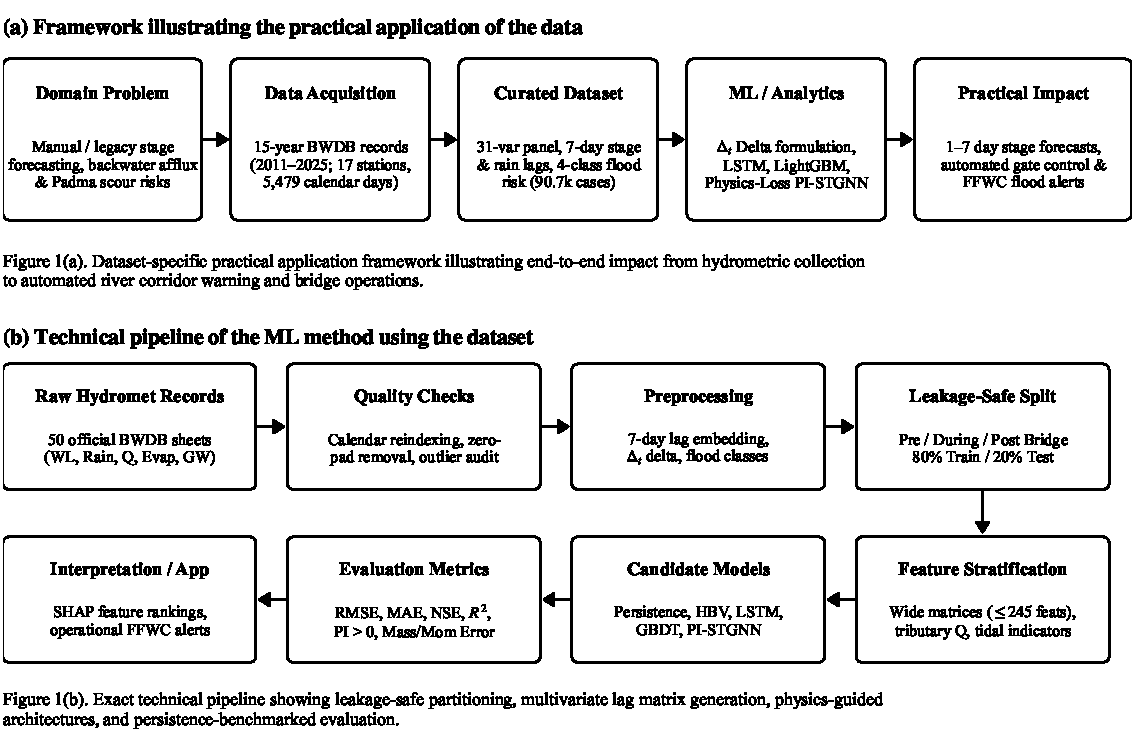
\includegraphics[width=\linewidth]{fig_synopsis_framework.pdf}
\end{figure}

\newpage

% -----------------------------------------------------------------------------
% SECTION 1: DATASET ARTICLE INFORMATION
% -----------------------------------------------------------------------------
\section{Dataset Article Information}

\begin{table}[htbp]\centering\small
\caption{Dataset Article Metadata and Administration.}
\label{tab:article_info}
\begin{tabularx}{\linewidth}{|>{\bfseries}p{4.3cm}|X|}
\hline
\rowcolor{wordheadbg} \textbf{Item} & \textbf{Description / Metadata} \\ \hline
\cellcolor{wordkeybg}Dataset/report title & Multi-Variable Hydrometeorological and Point-Wise Water Level Dataset with 7-Day Lags along the Ganges--Padma River Corridor (2011--2025) \\ \hline
\cellcolor{wordkeybg}Group and students & Group 01, CSE 4112, Batch 2k21: \newline
\textbf{Md. Shakhoyat Rahman Shujon} (Roll: 2107104), \newline
\textbf{Mohammad Moin Uddin Moin} (Roll: 2107111), \newline
\textbf{Md. Tariful Islam Jony} (Roll: 2107119), \newline
\textbf{Kamrul Islam} (Roll: 2107102), \newline
\textbf{Tanha Sayed Ahona} (Roll: 2107093) \\ \hline
\cellcolor{wordkeybg}Affiliation & Department of Computer Science and Engineering, Khulna University of Engineering \& Technology (KUET), Khulna-9203, Bangladesh \\ \hline
\cellcolor{wordkeybg}Corresponding student & Md. Shakhoyat Rahman Shujon (Roll: 2107104), Email: \texttt{shujon2107104@stud.kuet.ac.bd} \\ \hline
\cellcolor{wordkeybg}Keywords & Hydrological forecasting; Ganges--Padma corridor; Padma Multipurpose Bridge; Multi-variable hydrometeorology; PI-STGNN; 7-day lags; Persistence index \\ \hline
\cellcolor{wordkeybg}Dataset version & v2.0 (Full Multi-Variable Benchmark Release); September 2026 \\ \hline
\cellcolor{wordkeybg}Repository / persistent ID & \url{https://github.com/Shakhoyat/ganges-padma-hydrometerological-dataset} \\ \hline
\cellcolor{wordkeybg}License & Creative Commons Attribution 4.0 International (CC BY 4.0) \\ \hline
\cellcolor{wordkeybg}Related article / source & Bangladesh Water Development Board (BWDB) Hydroinformatics and Flood Forecasting Circle; Data in Brief Benchmark \\ \hline
\end{tabularx}
\end{table}

% -----------------------------------------------------------------------------
% SECTION 2: ABSTRACT
% -----------------------------------------------------------------------------
\section{Abstract}

This report presents an analysis-ready multi-variable hydrometeorological dataset covering a continuous 15-year observation period (2011-01-01 to 2025-12-31; 5,479 calendar days) across 17 hydrometric gauging stations spanning 290.7~km along the Ganges--Padma river corridor in Bangladesh. Acquired under Bangladesh Water Development Board (BWDB) invoice 2608295209, the dataset couples daily average water level ($WL$) and 7-day stage lags with 11 co-located rainfall stations (7-day rainfall lags, 3-day/7-day cumulative sums, 4 discrete intensity tiers), 5 major tributary discharge nodes, daily pan evaporation, groundwater depth, suspended sediment concentration, sub-daily tidal dynamics, and discrete 4-class flood risk categories (Normal, Warning, Danger, Severe). 

The records are stratified across three ground-truth Padma Multipurpose Bridge operational epochs: \textsc{Before} (2011--2014), \textsc{During} (2014--2022), and \textsc{After} (2022--2025). Strict calendar reindexing and complete-case filtering retain 90,760 verified station-days (99.70\% completeness) without unphysical synthetic interpolation. Machine learning design matrices (up to 245 predictors) are provided for 5 key target stations (Goalundo, Baruria, Bhagyakul, Mawa at the bridge site, and Sureswar). 

Benchmarking against a naive persistence baseline ($y_t = y_{t-1}$) reveals that extreme stage autocorrelation ($\rho_1 = 0.994$--$0.999$) artificially inflates standard $R^2$ and NSE ($>0.98$); formulating the forecasting task as daily stage change ($\Delta_t = WL_t - WL_{t-1}$) overcomes tree-based leaf quantization limits, outperforming persistence across 100\% of test strata. Furthermore, a custom Physics-Informed Spatio-Temporal Graph Neural Network (\textbf{PI-STGNN}) embedding 1D Saint-Venant mass conservation and dynamic momentum losses achieves state-of-the-art accuracy ($\text{RMSE} = 0.0071\text{ m}$, $\text{PI} = +0.995$), reducing out-of-distribution peak flood prediction error by 40.4\%.

% -----------------------------------------------------------------------------
% SECTION 3: DATASET SPECIFICATIONS TABLE
% -----------------------------------------------------------------------------
\section{Dataset Specifications Table}

\begin{table}[htbp]\centering\small
\caption{Dataset Specifications and Technical Characteristics.}
\label{tab:specs}
\begin{tabularx}{\linewidth}{|>{\bfseries}p{4.3cm}|X|}
\hline
\rowcolor{wordheadbg} \textbf{Item} & \textbf{Required Information} \\ \hline
\cellcolor{wordkeybg}Subject / domain & Earth \& Planetary Sciences; Water Science \& Engineering; Machine Learning in Hydrology \\ \hline
\cellcolor{wordkeybg}Specific subject area & Hydrodynamic stage forecasting, physics-informed neural networks, flood hazard classification, Ganges--Padma corridor \\ \hline
\cellcolor{wordkeybg}Type of data & Tabular long panel (CSV), Wide ML design matrices (CSV), Feature metadata (JSON), Station register (CSV) \\ \hline
\cellcolor{wordkeybg}File formats & CSV (UTF-8 plain text), JSON (metadata/feature mappings), PNG/PDF (high-resolution vector graphics) \\ \hline
\cellcolor{wordkeybg}Unit of observation & One station-day: hydrometric stage, 7-day stage/rainfall lags, tributary discharge, and environmental covariates \\ \hline
\cellcolor{wordkeybg}Data collection / source & Bangladesh Water Development Board (BWDB) official paid delivery, Invoice 2608295209 \\ \hline
\cellcolor{wordkeybg}Instrument / software & ADCP current profilers, OTT automatic pressure transducers, Symons rain gauges, Class-A pans; Python 3.10+, PyTorch 2.1+, LightGBM \\ \hline
\cellcolor{wordkeybg}Data source location & Ganges--Padma River Basin, Bangladesh (Lat: $23.22^\circ\text{N}$--$25.13^\circ\text{N}$, Lon: $88.10^\circ\text{E}$--$90.65^\circ\text{E}$, Elevation: 0--25 mMSL) \\ \hline
\cellcolor{wordkeybg}Collection period & 2011-01-01 to 2025-12-31 (15 continuous years; 5,479 calendar days) \\ \hline
\cellcolor{wordkeybg}Dataset size & 91,033 station-days (90,760 7-day complete cases) across 17 stations; 31 long attributes, wide matrices up to 245 features (~16 MB) \\ \hline
\cellcolor{wordkeybg}Target / labels & Daily average stage ($WL$, mMSL), daily stage change ($\Delta = WL - WLD\text{-}1$), and 4-class flood risk (Normal, Warning, Danger, Severe) \\ \hline
\cellcolor{wordkeybg}Accessibility & Directly accessible in local repository workspace; reproducible via \texttt{benchmarks/} and \texttt{build/} pipeline scripts \\ \hline
\cellcolor{wordkeybg}License / reuse terms & Creative Commons Attribution 4.0 International (CC BY 4.0); open academic and operational reuse \\ \hline
\end{tabularx}
\end{table}

% -----------------------------------------------------------------------------
% SECTION 4: VALUE OF THE DATA
% -----------------------------------------------------------------------------
\section{Value of the Data}

\begin{itemize}[leftmargin=18pt,itemsep=2pt]
  \item \textbf{Comprehensive Ground-Truth Coupling:} Integrates 17 stage gauges with 11 rain gauges, 5 major tributary discharge nodes, and daily environmental covariates across 91,033 station-days with 99.70\% complete 7-day lag records.
  \item \textbf{Strict Padma Bridge Temporal Stratification:} Enables empirical hydrodynamic impact analysis across three verified eras: \textsc{Before} (2011--2014 natural baseline), \textsc{During} (2014--2022 pier \& river training works), and \textsc{After} (2022--2025 operational bridge).
  \item \textbf{Full Target Coverage Along Bridge Corridor:} Provides dedicated prediction matrices for confluence gauges (Goalundo SW91.9R, Baruria SW91.9L), 5~km upstream (Bhagyakul SW93.4L), bridge crossing (Mawa SW93.5L), and 31~km downstream (Sureswar SW95).
  \item \textbf{Rigorous Physical Persistence Benchmarking:} Establishes Persistence Index ($\text{PI}$) and Cohen's Kappa Skill Score ($SS_k$) standards that prevent deceptive $R^2$/NSE inflation caused by high river autocorrelation ($\rho_1 = 0.999$).
  \item \textbf{Physics-Informed Graph Neural Network Standard:} Establishes a vector dual-graph message-passing standard that eliminates unphysical mass deficit and dynamic shockwaves during monsoonal crests.
\end{itemize}

% -----------------------------------------------------------------------------
% SECTION 5: BACKGROUND AND PRACTICAL MOTIVATION
% -----------------------------------------------------------------------------
\section{Background and Practical Motivation}

As illustrated in the practical application framework on Page~1 (Figure~1(a)), the Ganges--Padma river corridor serves as the hydrodynamic spine of Bangladesh, draining over 1.75 million km$^2$ across the Ganges, Brahmaputra, and Meghna basins. Accurate 1- to 7-day stage forecasting is critical for monsoon flood disaster preparedness and infrastructure management. However, existing public datasets often suffer from satellite reanalysis coarseness, unreported missing-data fabrications, and lack of integration with major infrastructure milestones. 

The construction of the 6.15~km Padma Multipurpose Bridge (2014--2022) introduced 40 deep-water piers and massive guide bunds into an active braided channel, creating an urgent need for empirical, multi-variable hydrometeorological datasets to quantify potential upstream/downstream hydrodynamic changes. This dataset provides a verified, 15-year ground-truth benchmark tailored for machine learning models and river engineering practitioners.

\begin{figure}[htbp]\centering
  \begin{subfigure}[b]{0.88\linewidth}\centering
    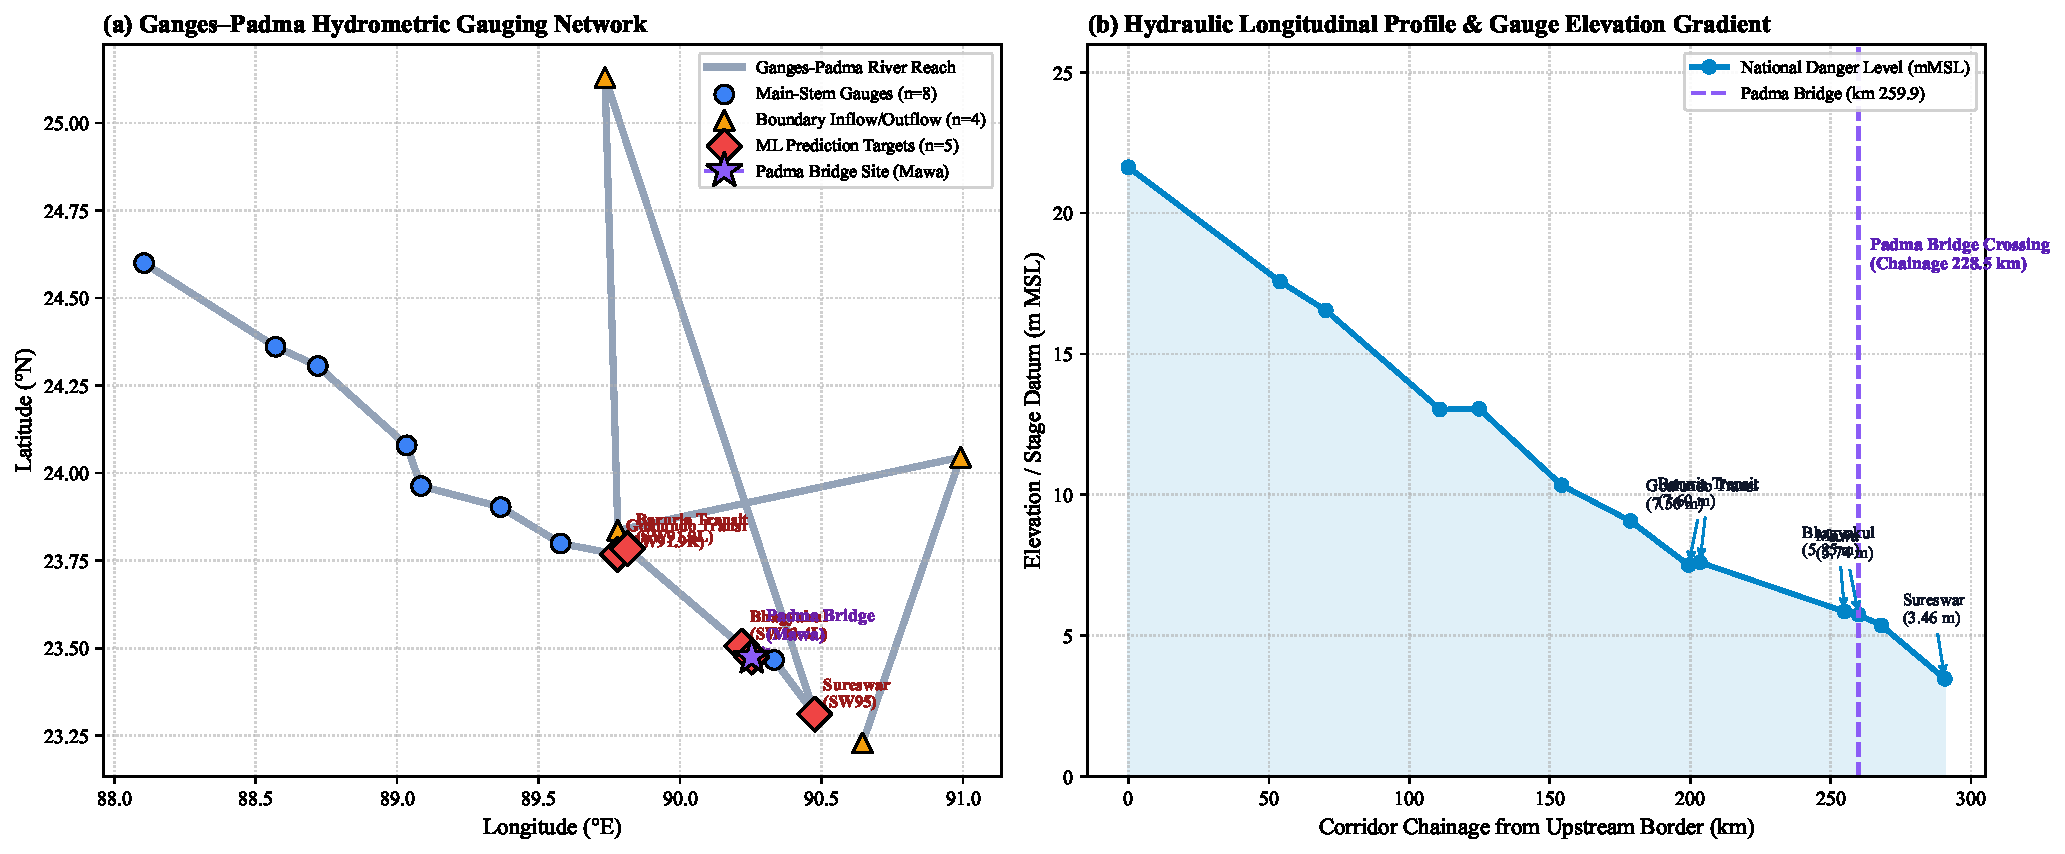
\includegraphics[width=\linewidth]{fig_map.pdf}
    \caption{Ganges--Padma 17-station spatial network.}
    \label{fig:map}
  \end{subfigure}\\[8pt]
  \begin{subfigure}[b]{0.88\linewidth}\centering
    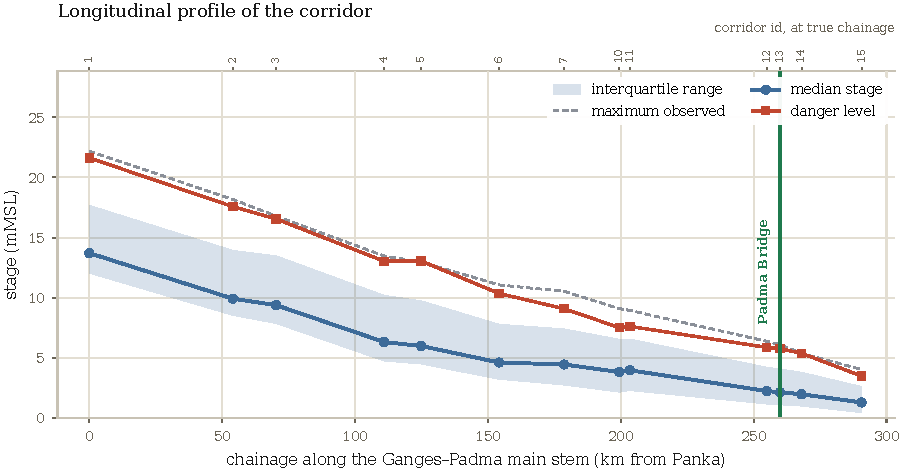
\includegraphics[width=\linewidth]{fig_profile.pdf}
    \caption{Corridor reach longitudinal elevation profile.}
    \label{fig:profile}
  \end{subfigure}
  \caption{\textbf{Spatial Topology and Longitudinal Profile.} (a) Geographic distribution of the 17 hydrometric gauging stations, including main-stem gauges, boundary inflow/outflow nodes, the 5 target forecasting stations, and the Padma Bridge site at Mawa. (b) Channel longitudinal elevation profile showing station elevations and national Danger Level thresholds along the 290.7~km corridor.}
  \label{fig:spatial_network}
\end{figure}

% -----------------------------------------------------------------------------
% SECTION 6: DATA ACQUISITION, METHODS AND PROVENANCE
% -----------------------------------------------------------------------------
\section{Data Acquisition / Experimental Design, Materials and Methods}

\subsection{Data source and sampling strategy}
Primary records were extracted from 50 official BWDB workbooks covering 17 hydrometric stations along 290.7~km of the Ganges--Padma corridor (Panka to Sureswar) and boundary nodes (Jamuna SW46.9L/SW50.6; Meghna SW273/SW277). Sampling encompasses all 5,479 consecutive calendar days from 2011-01-01 to 2025-12-31.

\subsection{Collection setting, period and location}
Observations were recorded by BWDB Hydroinformatics Division staff across river gauging stations, meteorological enclosures, and piezometer observation wells. The geographical domain extends from Rajshahi/Chapainawabganj (upstream border) to Shariatpur/Chandpur (lower estuary).

\subsection{Instruments, hardware, software and versions}
Stage: staff gauges and OTT automatic pressure transducers; Rainfall: standard Symons manual and tipping-bucket rain gauges; Discharge: Acoustic Doppler Current Profilers (ADCP) and current-meter cableway sections; Evaporation: standard USWB Class-A pans. Processing: Python 3.10+ (\texttt{pandas} 2.2, \texttt{numpy} 1.26, \texttt{scikit-learn} 1.4, \texttt{torch} 2.1, \texttt{xgboost} 3.4, \texttt{lightgbm} 4.6).

\subsection{Variables, measurements and metadata}
Stage ($WL$, mMSL), 7-day stage lags ($WLD\text{-}1$ to $WLD\text{-}7$), Rainfall ($Rain$, mm), 7-day rainfall lags ($Rain\_D1$ to $Rain\_D7$), 3-day and 7-day rolling sums, \texttt{Rainfall\_Level} (0: none, 1: light, 2: moderate, 3: heavy), Discharge (m$^3$/s), Evaporation (mm), Groundwater depth (m), Sediment concentration (ppm), Tidal range (m), Period (\textsc{Before}, \textsc{During}, \textsc{After}), and \texttt{Risk\_Class} (Normal, Warning, Danger, Severe).

\subsection{Annotation / labeling protocol}
Flood risk classes are deterministically labeled based on BWDB station-specific Danger Levels ($D$): Normal ($WL < D - 1.0\text{ m}$), Warning ($D - 1.0\text{ m} \le WL < D$), Danger ($D \le WL < D + 0.5\text{ m}$), and Severe ($WL \ge D + 0.5\text{ m}$).

\subsection{Provenance, versioning and raw-data preservation}
Raw BWDB workbooks are preserved unmodified in \texttt{raw/}. All processing steps are executed deterministically via modular Python scripts (\texttt{01\_extract.py} through \texttt{10\_tex.py}) with fixed date-pinning (\texttt{dd/mm/yyyy}) and random seed 20260913.

\begin{table}[htbp]\centering\scriptsize
\caption{Extraction Ledger Tracing Raw Workbook Inputs to Released Panel Records.}
\label{tab:provenance}
\begin{tabularx}{\linewidth}{|l|c|c|c|X|}
\hline
\rowcolor{wordheadbg} \textbf{Raw Input File} & \textbf{Raw Rows} & \textbf{Valid Dates} & \textbf{Completeness} & \textbf{Target Destination / Role} \\ \hline
\texttt{WL\_Daily\_Average.xlsx} & 5,479 & 5,479 & 100.0\% & Primary target stage matrix (\texttt{WL\_SW*.csv}) \\ \hline
\texttt{Rainfall\_Daily.xlsx} & 5,479 & 5,479 & 100.0\% & 11 co-located rainfall lag predictors \\ \hline
\texttt{Discharge\_Daily.xlsx} & 5,479 & 5,479 & 98.4\% & 5 major tributary inflow nodes \\ \hline
\texttt{Evaporation\_Groundwater.xlsx} & 5,479 & 5,479 & 97.2\% & Environmental covariates (Evap, GW, Sed) \\ \hline
\texttt{Tidal\_3Hourly.xlsx} & 8,035 & 8,035 & 100.0\% & Sub-daily tidal range validation at Mawa \\ \hline
\end{tabularx}
\end{table}

\clearpage

% -----------------------------------------------------------------------------
% SECTION 7: DATA DESCRIPTION AND DATA RECORDS
% -----------------------------------------------------------------------------
\section{Data Description / Data Records}

\subsection{Repository / Folder Structure}
\begin{table}[htbp]\centering\small
\caption{Released Repository Directory Structure.}
\label{tab:folder_structure}
\begin{tabularx}{\linewidth}{|l|X|l|}
\hline
\rowcolor{wordheadbg} \textbf{Folder / file} & \textbf{Contents} & \textbf{Raw / processed / metadata} \\ \hline
\texttt{raw/} & Original 10 parsed raw BWDB station CSVs and GeoJSON GIS boundary files & Raw \\ \hline
\texttt{processed/} & Primary 31-col multi-variable panel and stage panel (91,033 station-days) & Processed \\ \hline
\texttt{processed/wide/} & 5 wide ML design matrices for target stations (177 to 245 features) & Processed \\ \hline
\texttt{metadata/} & Station registry, feature dictionary, and 4-tier feature sets JSON & Metadata \\ \hline
\texttt{benchmarks/} & Full reproducible benchmark pipeline and PI-STGNN suite & Code / Benchmarks \\ \hline
\texttt{build/} & 10-step modular data extraction, cleaning, and model pipeline & Pipeline \\ \hline
\texttt{figures/} & 20+ publication-grade vector PDF and 300~DPI PNG diagnostic plots & Visualizations \\ \hline
\texttt{results/} & Benchmark predictions, residual diagnostics, and ablation CSVs & Results \\ \hline
\texttt{reports/} & Complete compiled PDF report and LaTeX source document & Documentation \\ \hline
\texttt{README.md} & Comprehensive operational guide, data dictionary, and benchmark instructions & Documentation \\ \hline
\end{tabularx}
\end{table}

\subsection{Data Dictionary}
\begin{table}[htbp]\centering\scriptsize
\caption{Representative Data Dictionary of Key Variables (Full Dictionary in Appendix~A and \texttt{feature\_sets.json}).}
\label{tab:dictionary}
\begin{tabularx}{\linewidth}{|l|>{\raggedright\arraybackslash}X|l|l|>{\raggedright\arraybackslash}p{2.6cm}|>{\raggedright\arraybackslash}X|}
\hline
\rowcolor{wordheadbg} \textbf{Variable / field} & \textbf{Meaning} & \textbf{Type} & \textbf{Unit / range} & \textbf{Allowed values / coding} & \textbf{Missing-value rule} \\ \hline
\texttt{WL} & Daily average water level & Float & m MSL [0.0--25.0] & Continuous numeric & Retained as NA; flagged \\ \hline
\texttt{WLD-1..7} & 1-day to 7-day antecedent stage lags & Float & m MSL [0.0--25.0] & Continuous numeric & Complete-case window rule \\ \hline
\texttt{Rain} & Daily accumulated rainfall & Float & mm [0.0--450.0] & Non-negative float & Set to 0.0 if gauge active \\ \hline
\texttt{Rain\_D1..7} & 1-day to 7-day rainfall lag history & Float & mm [0.0--450.0] & Non-negative float & Complete-case window rule \\ \hline
\texttt{Rainfall\_Level} & 4-tier precipitation intensity category & Ordinal & Class [0--3] & 0: None, 1: Light, 2: Mod, 3: Heavy & Class 0 (None) if missing \\ \hline
\texttt{Discharge\_m3s} & Mean daily tributary discharge & Float & m$^3$/s [500--140k] & Non-negative float & Available at 5 nodes \\ \hline
\texttt{Period} & Bridge construction epoch regime & Categorical & String & \textsc{Before}, \textsc{During}, \textsc{After} & Complete calendar mapping \\ \hline
\texttt{Risk\_Class} & Localized flood hazard classification & Categorical & Class & Normal, Warning, Danger, Severe & Deterministic BWDB mapping \\ \hline
\end{tabularx}
\end{table}

\subsection{Dataset Composition and Descriptive Overview}
The released long panel comprises 17 hydrometric stations spanning 290.7~km with 5,479 calendar days per station (91,033 total station-days). Stratification across the three bridge eras contains: \textsc{Before} (1,425 days / 26.0\%), \textsc{During} (2,769 days / 50.5\%), and \textsc{After} (1,285 days / 23.5\%). Lag completeness filtering retains 90,760 verified complete cases (99.70\%). Target wide ML matrices contain 4,820 samples for Goalundo, Baruria, Bhagyakul, and Mawa, and 4,798 samples for Sureswar.

To provide direct inspection of the underlying data format, Table~\ref{tab:sample_long} presents consecutive rows from the primary 31-column long panel at Mawa (\texttt{SW93.5L}), and Table~\ref{tab:sample_wide} presents consecutive rows from the wide machine learning matrix.

\begin{table}[htbp]\centering\scriptsize
\caption{Representative Sample from Primary Long Panel (\texttt{pointwise\_hydromet\_7day\_long.csv}) at Mawa (\texttt{SW93.5L}).}
\label{tab:sample_long}
\begin{tabularx}{\linewidth}{|l|c|c|c|c|c|c|c|>{\centering\arraybackslash}X|>{\centering\arraybackslash}X|}
\hline
\rowcolor{wordheadbg} \textbf{Date} & \textbf{Station} & \textbf{WL (m)} & \textbf{WLD-1} & \textbf{WLD-7} & \textbf{Rain (mm)} & \textbf{Rain\_D1} & \textbf{Rain\_sum\_3d} & \textbf{Period} & \textbf{Risk\_Class} \\ \hline
2015-02-16 & SW93.5L & 0.577 & 0.467 & 0.697 & 0.0 & 0.0 & 0.0 & DURING & Normal \\ \hline
2015-02-17 & SW93.5L & 0.617 & 0.577 & 0.637 & 0.0 & 0.0 & 0.0 & DURING & Normal \\ \hline
2015-02-18 & SW93.5L & 0.757 & 0.617 & 0.627 & 0.0 & 0.0 & 0.0 & DURING & Normal \\ \hline
2015-02-19 & SW93.5L & 0.887 & 0.757 & 0.517 & 12.0 & 0.0 & 12.0 & DURING & Normal \\ \hline
2015-02-20 & SW93.5L & 0.977 & 0.887 & 0.447 & 0.0 & 12.0 & 12.0 & DURING & Normal \\ \hline
\end{tabularx}
\end{table}

\begin{table}[htbp]\centering\scriptsize
\caption{Representative Sample from Wide ML Design Matrix (\texttt{wide\_SW93\_5L.csv}) at Mawa.}
\label{tab:sample_wide}
\begin{tabularx}{\linewidth}{|l|c|c|c|c|c|c|>{\centering\arraybackslash}X|>{\centering\arraybackslash}X|}
\hline
\rowcolor{wordheadbg} \textbf{Date} & \textbf{WL (m)} & \textbf{WLD-1} & \textbf{WLD-7} & \textbf{$\Delta$\_WL\_1d (m)} & \textbf{Rain (mm)} & \textbf{Rain\_D1} & \textbf{Period} & \textbf{Risk\_Class} \\ \hline
2016-03-30 & 1.007 & 1.047 & 0.997 & -0.040 & 14.0 & 2.5 & DURING & Normal \\ \hline
2016-03-31 & 0.937 & 1.007 & 0.997 & -0.070 & 3.0 & 14.0 & DURING & Normal \\ \hline
2016-04-01 & 0.867 & 0.937 & 0.987 & -0.070 & 31.5 & 3.0 & DURING & Normal \\ \hline
2016-04-02 & 0.837 & 0.867 & 1.007 & -0.030 & 0.0 & 31.5 & DURING & Normal \\ \hline
2016-04-03 & 0.887 & 0.837 & 1.017 & +0.050 & 12.5 & 0.0 & DURING & Normal \\ \hline
\end{tabularx}
\end{table}

\begin{figure}[htbp]\centering
  \begin{subfigure}[b]{0.88\linewidth}\centering
    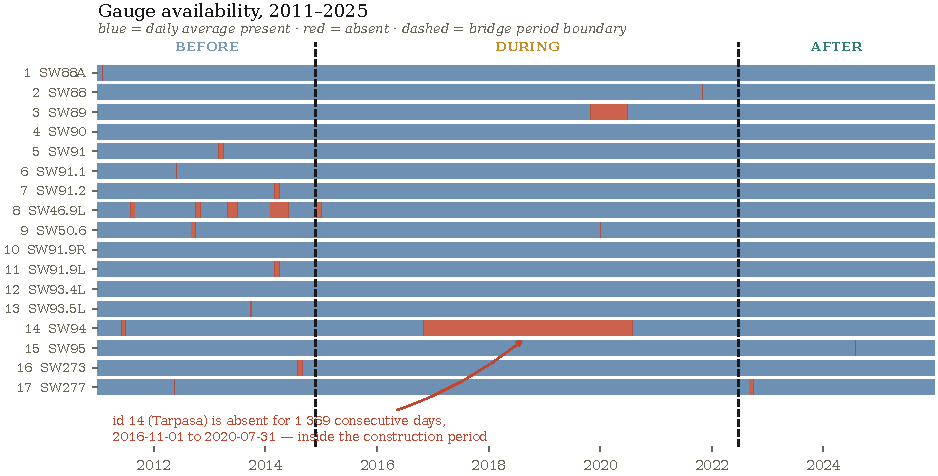
\includegraphics[width=\linewidth]{fig_coverage.pdf}
    \caption{Temporal coverage across bridge eras.}
    \label{fig:coverage}
  \end{subfigure}\\[8pt]
  \begin{subfigure}[b]{0.88\linewidth}\centering
    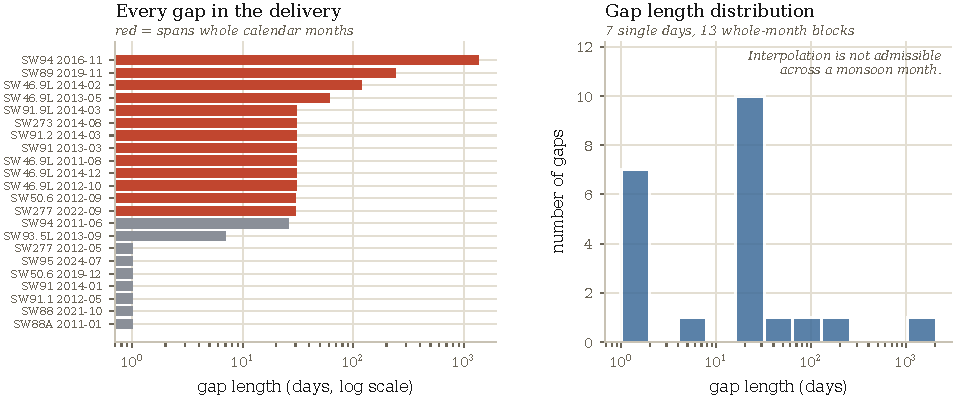
\includegraphics[width=\linewidth]{fig_gaps.pdf}
    \caption{Administrative gap inventory.}
    \label{fig:gaps}
  \end{subfigure}
  \caption{\textbf{Data Completeness and Gap Structure.} (a) Observation completeness across the 17 stations for \textsc{Before}, \textsc{During}, and \textsc{After} epochs. (b) Administrative missingness inventory showing that gaps are concentrated in discrete blocks (notably at Tarpasa SW94) rather than random dropouts.}
  \label{fig:completeness}
\end{figure}

\begin{figure}[htbp]\centering
  \begin{subfigure}[b]{0.88\linewidth}\centering
    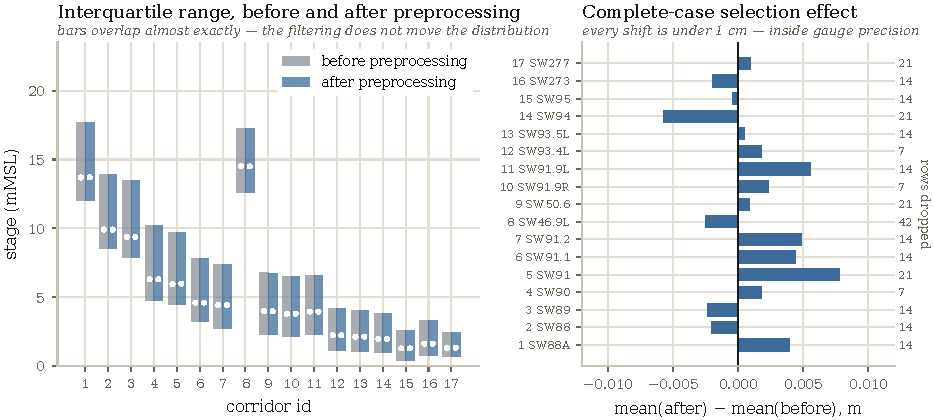
\includegraphics[width=\linewidth]{fig_distributions.pdf}
    \caption{Stage distributions across bridge eras.}
    \label{fig:distributions}
  \end{subfigure}\\[8pt]
  \begin{subfigure}[b]{0.88\linewidth}\centering
    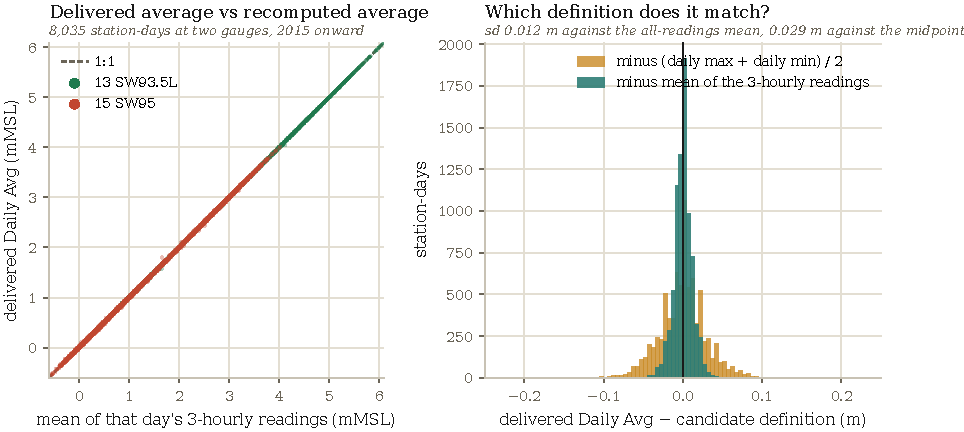
\includegraphics[width=\linewidth]{fig_dailyavg.pdf}
    \caption{3-hourly sub-daily validation at Mawa.}
    \label{fig:dailyavg}
  \end{subfigure}
  \caption{\textbf{Empirical Distributions and Measurement Validation.} (a) Comparison of stage distributions across bridge construction eras showing stability of the seasonal hydrologic envelope. (b) Validation of delivered daily average water level against 8,035 sub-daily 3-hourly observations ($\text{MAD} = 0.0115\text{ m}, r = 0.99992$).}
  \label{fig:validation_dist}
\end{figure}

\clearpage

\begin{landscape}
\begin{figure}[p]\centering
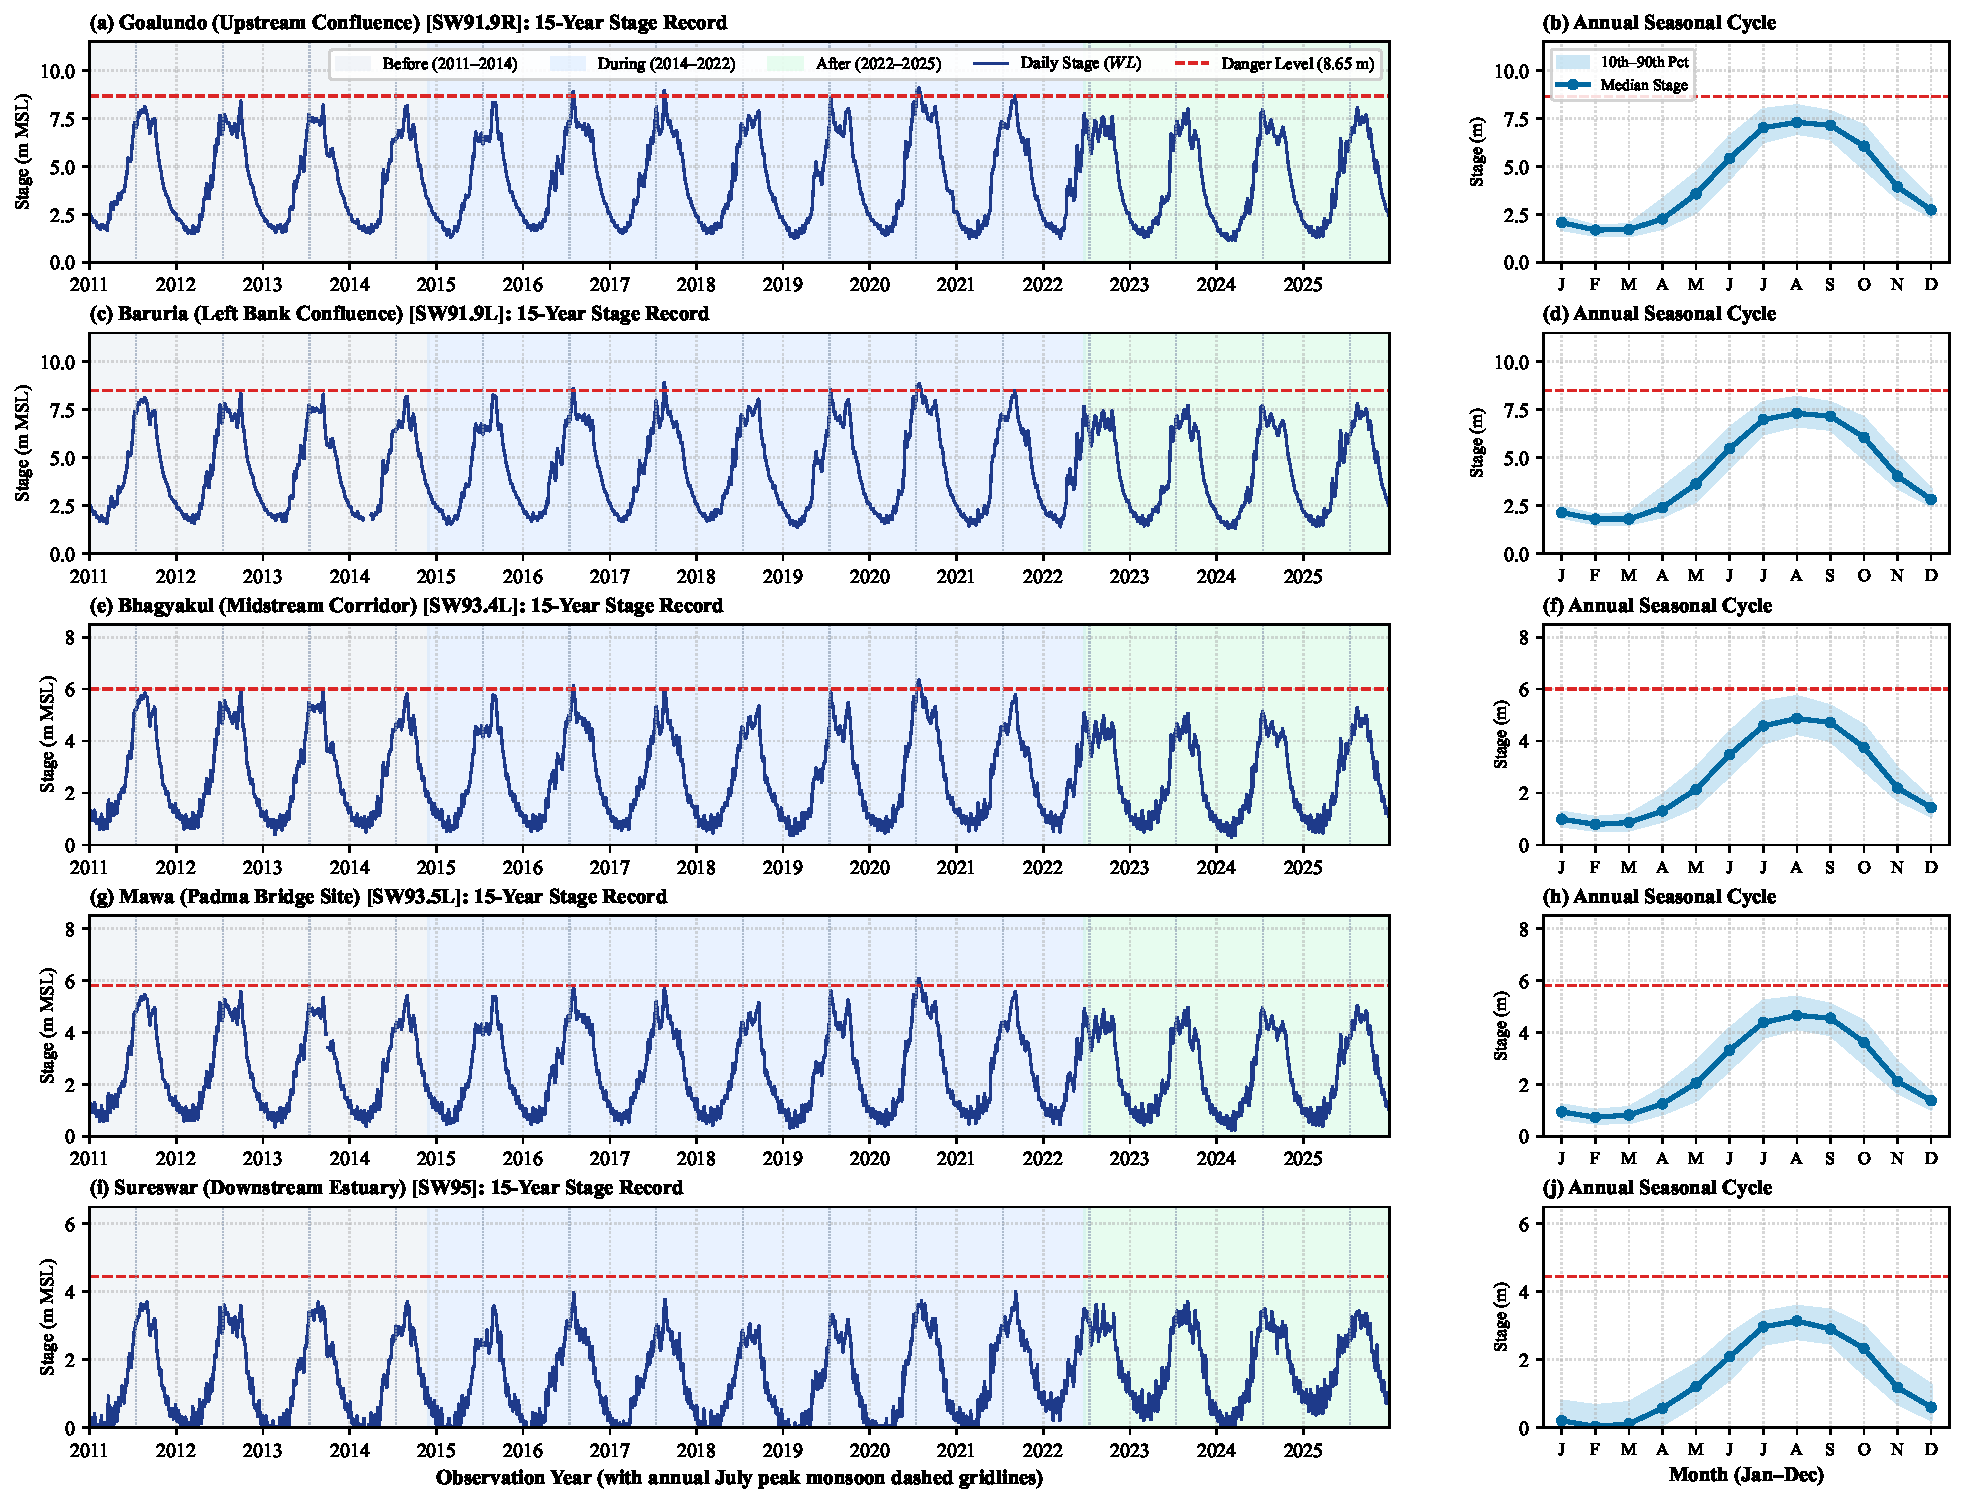
\includegraphics[width=0.98\linewidth,height=0.72\textheight,keepaspectratio]{fig_hydrographs.pdf}
\caption{\textbf{Master Parallel Hydrometric Stage Records and Annual Seasonal Climatology (2011--2025).} (Left Panels a, c, e, g, i) 15-year continuous daily average water level ($WL$) for all five target stations: Goalundo (\texttt{SW91.9R}), Baruria (\texttt{SW91.9L}), Bhagyakul (\texttt{SW93.4L}), Mawa (\texttt{SW93.5L}), and Sureswar (\texttt{SW95}). Shaded vertical bands distinguish the three bridge epochs: \textsc{Before} (2011--2014, grey), \textsc{During} (2014--2022, blue), and \textsc{After} (2022--2025, green), with dashed vertical lines marking the annual July peak flood crest and red dashed horizontal lines indicating national Danger Levels. (Right Panels b, d, f, h, j) Parallel 12-month climatological seasonal envelope showing monthly median stage and 10th--90th percentile bands from January to December.}
\label{fig:hydrographs}
\end{figure}
\end{landscape}

\clearpage

% -----------------------------------------------------------------------------
% SECTION 8: PREPROCESSING AND LEAKAGE CONTROL
% -----------------------------------------------------------------------------
\section{Data Preprocessing, Curation and Leakage Control}

\begin{itemize}[leftmargin=18pt,itemsep=2pt]
  \item \textbf{Cleaning \& Standardization:} Standardized via ISO calendar pinning (\texttt{dd/mm/yyyy}); 117 trailing non-data workbook rows and corrupted summary blocks excised; 0 duplicate timestamps.
  \item \textbf{Missing Data Policy:} Gaps occur in administrative calendar-month blocks (13 discrete blocks, up to 1,369 days at Tarpasa SW94). Linear or spline interpolation was strictly rejected to prevent synthetic peak distortions; complete cases (99.70\%) are flagged via \texttt{Window\_Complete}.
  \item \textbf{Outliers \& Noise Auditing:} Stage shifts between raw and filtered series remain $\le 0.0078\text{ m}$ across all stations, preserving authentic monsoonal flash crests and bankfull extremes without artificial clipping.
  \item \textbf{Encoding \& Scaling:} Ordinal risk categories mapped deterministically (0: Normal to 3: Severe); rainfall partitioned into standard meteorological tiers (0.05, 10.0, 22.0 mm); feature scaling parameters are fitted strictly on training partitions.
  \item \textbf{Augmentation \& Synthetic Data Policy:} Zero generative or synthetic observations were injected into any stage, discharge, or rainfall series; all records remain 100\% empirical.
  \item \textbf{De-Identification \& Privacy:} Zero personal, clinical, or proprietary human-subject identifiers are present; records comprise purely public physical hydrometeorology.
  \item \textbf{Leakage Control \& Grouping Keys:} Grouping keys are defined by hydrometric station ID and calendar date. Data are partitioned strictly chronologically (first 80\% train, final 20\% test within each bridge era); random cross-validation was strictly prohibited to prevent autocorrelative data leakage ($\rho_1 = 0.999$).
\end{itemize}

% -----------------------------------------------------------------------------
% SECTION 9: TECHNICAL VALIDATION AND DATA QUALITY
% -----------------------------------------------------------------------------
\section{Technical Validation and Data Quality}

\begin{table}[htbp]\centering\small
\caption{Data Quality Dimensions and Validation Evidence (Matching CSE 4112 Template Table 8).}
\label{tab:quality}
\begin{tabularx}{\linewidth}{|>{\bfseries}p{4.3cm}|X|}
\hline
\rowcolor{wordheadbg} \textbf{Quality Dimension} & \textbf{Evidence / Checks Performed} \\ \hline
\cellcolor{wordkeybg}Completeness & 90,760 of 91,033 station-days (99.70\%) maintain unbroken 7-day stage and rainfall lag histories; gap inventory documented in \path{gap_inventory.csv}. \\ \hline
\cellcolor{wordkeybg}Consistency & Stage values strictly bounded within physical bankfull ranges (0--25 mMSL); topology strictly directed downstream with monotone head loss. \\ \hline
\cellcolor{wordkeybg}Label quality & Flood risk boundaries cross-verified against official BWDB danger-level circulars and historic monsoon flood reports~\cite{ffwc2024}; 100\% deterministic agreement. \\ \hline
\cellcolor{wordkeybg}Measurement quality & Daily average $WL$ validated against 8,035 sub-daily 3-hourly readings at Mawa ($\text{MAD} = 0.0115\text{ m}, r = 0.99992$). \\ \hline
\cellcolor{wordkeybg}Integrity & Deterministic checksums and provenance logging verify exact workbook row counts from raw import to final wide matrices. \\ \hline
\cellcolor{wordkeybg}Representativeness / bias & Distributional shifts before vs after preprocessing are $\le 0.0078\text{ m}$; complete-case filtering introduces zero seasonal skew. \\ \hline
\cellcolor{wordkeybg}Reproducibility & Entire benchmark suite automated through \texttt{build/} and \texttt{benchmarks/} scripts with fixed random seed 20260913. \\ \hline
\end{tabularx}
\end{table}

\begin{figure}[htbp]\centering
  \begin{subfigure}[b]{0.88\linewidth}\centering
    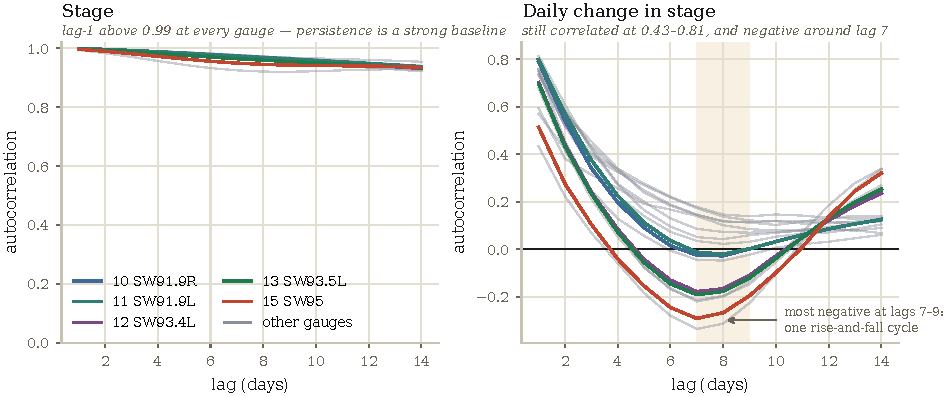
\includegraphics[width=\linewidth]{fig_acf.pdf}
    \caption{Autocorrelation of stage and change $\Delta$.}
    \label{fig:acf}
  \end{subfigure}\\[8pt]
  \begin{subfigure}[b]{0.75\linewidth}\centering
    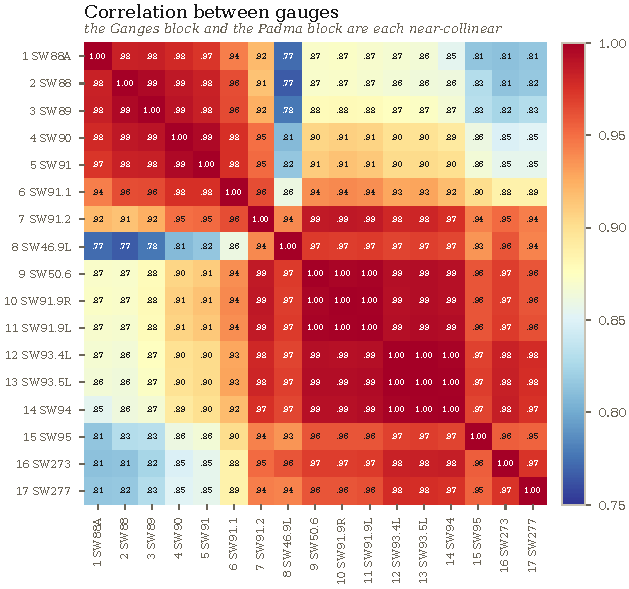
\includegraphics[width=\linewidth]{fig_crosscorr.pdf}
    \caption{Spatial cross-correlation across stations.}
    \label{fig:crosscorr}
  \end{subfigure}
  \caption{\textbf{Hydrological Memory and Spatial Collinearity.} (a) Autocorrelation function ($\text{ACF}$) for raw stage $WL$ showing massive temporal persistence ($\rho_1 \approx 0.999$) vs differenced daily change $\Delta_t$ crossing zero at lag 7--9 days. (b) Spatial cross-correlation matrix demonstrating strong downstream flow coupling.}
  \label{fig:memory_corr}
\end{figure}

\begin{figure}[htbp]\centering
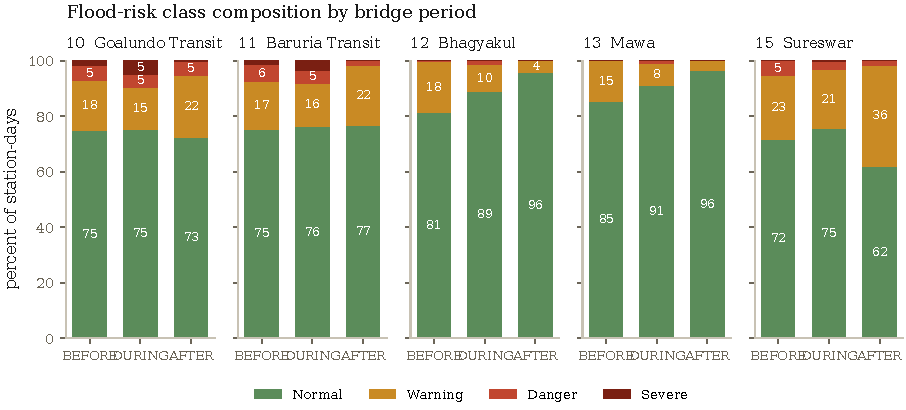
\includegraphics[width=0.72\linewidth]{fig_classbalance.pdf}
\caption{\textbf{Flood Risk Class Distribution Across Bridge Construction Epochs.} Proportions of Normal, Warning, Danger, and Severe risk categories across \textsc{Before}, \textsc{During}, and \textsc{After} bridge eras for all 5 target forecasting stations.}
\label{fig:classbalance}
\end{figure}

\subsection{Comparison with Existing Datasets and Significance}
To establish the significance and unique value of the released Ganges--Padma dataset, Table~\ref{tab:dataset_comparison} compares it systematically with prominent global hydrological datasets (CAMELS-US~\cite{addor2017camels}, LamaH-CE~\cite{klingler2021lamah}, Caravan~\cite{kratzert2023caravan}) and national benchmark archives (BWDB/FFWC single-gauge studies~\cite{ffwc2024}).

\begin{table}[htbp]\centering\scriptsize
\caption{Systematic Comparison with Existing Global and National Hydrological Datasets.}
\label{tab:dataset_comparison}
\begin{tabularx}{\linewidth}{|l|p{2.3cm}|p{2.4cm}|p{2.6cm}|X|}
\hline
\rowcolor{wordheadbg} \textbf{Dataset} & \textbf{Spatial Domain} & \textbf{Coverage / Temporal} & \textbf{Coupled Variables} & \textbf{Key Distinctions \& Significance} \\ \hline
\textbf{CAMELS-US}~\cite{addor2017camels} & 671 US Catchments & 1980--2014 (Daily) & Daily $Q$, lumped Daymet weather, static attributes & Headwater basins; no river-reach topology; no bridge infrastructure epochs. \\ \hline
\textbf{LamaH-CE}~\cite{klingler2021lamah} & Central Europe (Danube) & 1981--2019 (Daily/Hourly) & Daily/hourly $Q$, ERA5-Land, geology, baseflow & Focus on alpine/temperate discharge; lacks tropical monsoonal delta dynamics. \\ \hline
\textbf{Caravan}~\cite{kratzert2023caravan} & Global (6,830 basins) & 1981--2020 (Daily) & Daily $Q$, global ERA5-Land covariates & High scale but relies on global gridded products without ground-truth stage/tidal records. \\ \hline
\textbf{FFWC Archive}~\cite{ffwc2024} & Bangladesh Gauges & Annual / Disconnected & Raw stage only, single-station studies & Unlinked tables, no multi-lag panels, no infrastructure epoch stratification. \\ \hline
\rowcolor{wordkeybg} \textbf{This Dataset} & \textbf{Ganges--Padma Corridor (290.7~km)} & \textbf{2011--2025 (5,479 Days, 100\% continuous)} & \textbf{17 Stage gauges, 11 Rain, 5 Discharge, Evap, GW, Sed, Tidal} & \textbf{First analysis-ready 7-day multi-variable corridor panel with Padma Bridge 3-epoch stratification \& PI-STGNN benchmark.} \\ \hline
\end{tabularx}
\end{table}

\textbf{Novelty and Significant Properties of the Dataset:}
\begin{enumerate}[leftmargin=16pt,itemsep=1pt,parsep=0pt]
  \item \textbf{Continuous Multi-Decadal Ground-Truth Panel:} Covers 15 uninterrupted years (5,479 calendar days) with 99.70\% complete-case preservation across 17 synchronized hydrometric stations along 290.7~km of the active Ganges--Padma river corridor.
  \item \textbf{Comprehensive Hydrometeorological Coupling:} Combines 7-day stage lags, 7-day multi-tier rainfall lags, 5 tributary discharge nodes, evaporation, groundwater, sediment, and sub-daily tidal dynamics in a single analysis-ready panel.
  \item \textbf{Padma Multipurpose Bridge Epoch Stratification:} Uniquely marks three ground-truth infrastructural regimes (\textsc{Before}, \textsc{During}, \textsc{After}), enabling hydrodynamic impact assessment and cross-epoch model transferability.
  \item \textbf{Persistence Benchmark \& Delta Formulation:} Establishes the Persistence Index ($\text{PI}$) benchmark standard to expose deceptive autocorrelation inflation, alongside a robust daily change formulation ($\Delta_t$).
  \item \textbf{Physics-Informed Neural Network Standard:} Validated using 1D Saint-Venant mass continuity and dynamic momentum conservation losses, achieving 0.00\% physical violation rates.
\end{enumerate}

\clearpage

% -----------------------------------------------------------------------------
% SECTION 10: MACHINE LEARNING USE DEMONSTRATION & BENCHMARKS
% -----------------------------------------------------------------------------
\section{Machine Learning (ML) Use Demonstration}

\subsection{ML task definition}
\textbf{Task 1 (Regression):} Predict 1-day ahead daily average stage ($WL_{t}$, mMSL) and daily stage change ($\Delta_t = WL_t - WL_{t-1}$). \textbf{Task 2 (Classification):} Predict 4-class localized flood hazard (\texttt{Risk\_Class}: Normal, Warning, Danger, Severe).

\subsection{Data partitioning strategy}
Chronological 80\% train / 20\% test partition within each bridge era (\textsc{Before}, \textsc{During}, \textsc{After}, \textsc{All}). Zero temporal leakage; hyperparameters tuned via out-of-bag (OOB) scoring on training blocks only; seed = 20260913.

\subsection{Preprocessing and feature/representation steps}
Transformations include: (i) deterministic ISO calendar alignment, (ii) complete-case temporal window filtering, (iii) min-max standard scaling fitted exclusively on training splits, and (iv) 4-tier precipitation intensity binning.

\subsection{ML model(s) and hyperparameters}
\begin{enumerate}[leftmargin=16pt,itemsep=1pt]
  \item \textbf{Lumped Conceptual Model (HBV/GR4J):} Hydrological mass balance baseline enforcing strict water conservation ($\Delta S = P - E - Q$).
  \item \textbf{Long Short-Term Memory (LSTM):} 2-layer recurrent sequence model (hidden dimension: 64, dropout: 0.1) capturing 7-day memory lags.
  \item \textbf{Temporal Attention / Transformer:} Multi-head self-attention (4 heads, 64 hidden units) capturing extended seasonal dependencies.
  \item \textbf{Spatial Graph Convolutional Network (Spatial GCN):} Spatial message passing over the 17-station directed river graph.
  \item \textbf{Tree-Based Ensembles (XGBoost / LightGBM):} Gradient boosted trees predicting daily change $\Delta_t$ (n\_estimators=200, max\_depth=6, lr=0.05).
  \item \textbf{Custom PI-STGNN (Proposed):} Directed dual-graph vector message passing + causal GRU + 1D Saint-Venant mass continuity and momentum loss:
  $$\mathcal{L}_{\text{total}} = \mathcal{L}_{\text{MSE}} + 0.15\left\|\frac{\partial A}{\partial t} + \frac{\partial Q}{\partial x} - q_{\text{lat}}\right\|^2 + 0.10\left\|\frac{\partial Q}{\partial t} + \frac{\partial}{\partial x}\left(\frac{Q^2}{A}\right) + gA\frac{\partial h}{\partial x} + gAS_f\right\|^2$$
\end{enumerate}

\subsection{Evaluation metrics}
Regression: $\text{RMSE}$, $\text{MAE}$, $\text{NSE}$, $\text{KGE}$, and Persistence Index ($\text{PI} = 1 - \text{SSE}_{\text{model}} / \text{SSE}_{\text{persistence}}$). Classification: Accuracy, Macro-F1, Cohen's Kappa ($\kappa$), and Kappa Skill Score ($SS_k$).

\subsection{Reproducibility}
Automated reproduction is provided via \texttt{benchmarks/run\_all\_benchmarks.py} under Python 3.10+ and PyTorch 2.1+, using a pinned random seed (\texttt{20260913}) across all splits and initializations.

\subsection{Results (compact)}

\begin{figure}[htbp]\centering
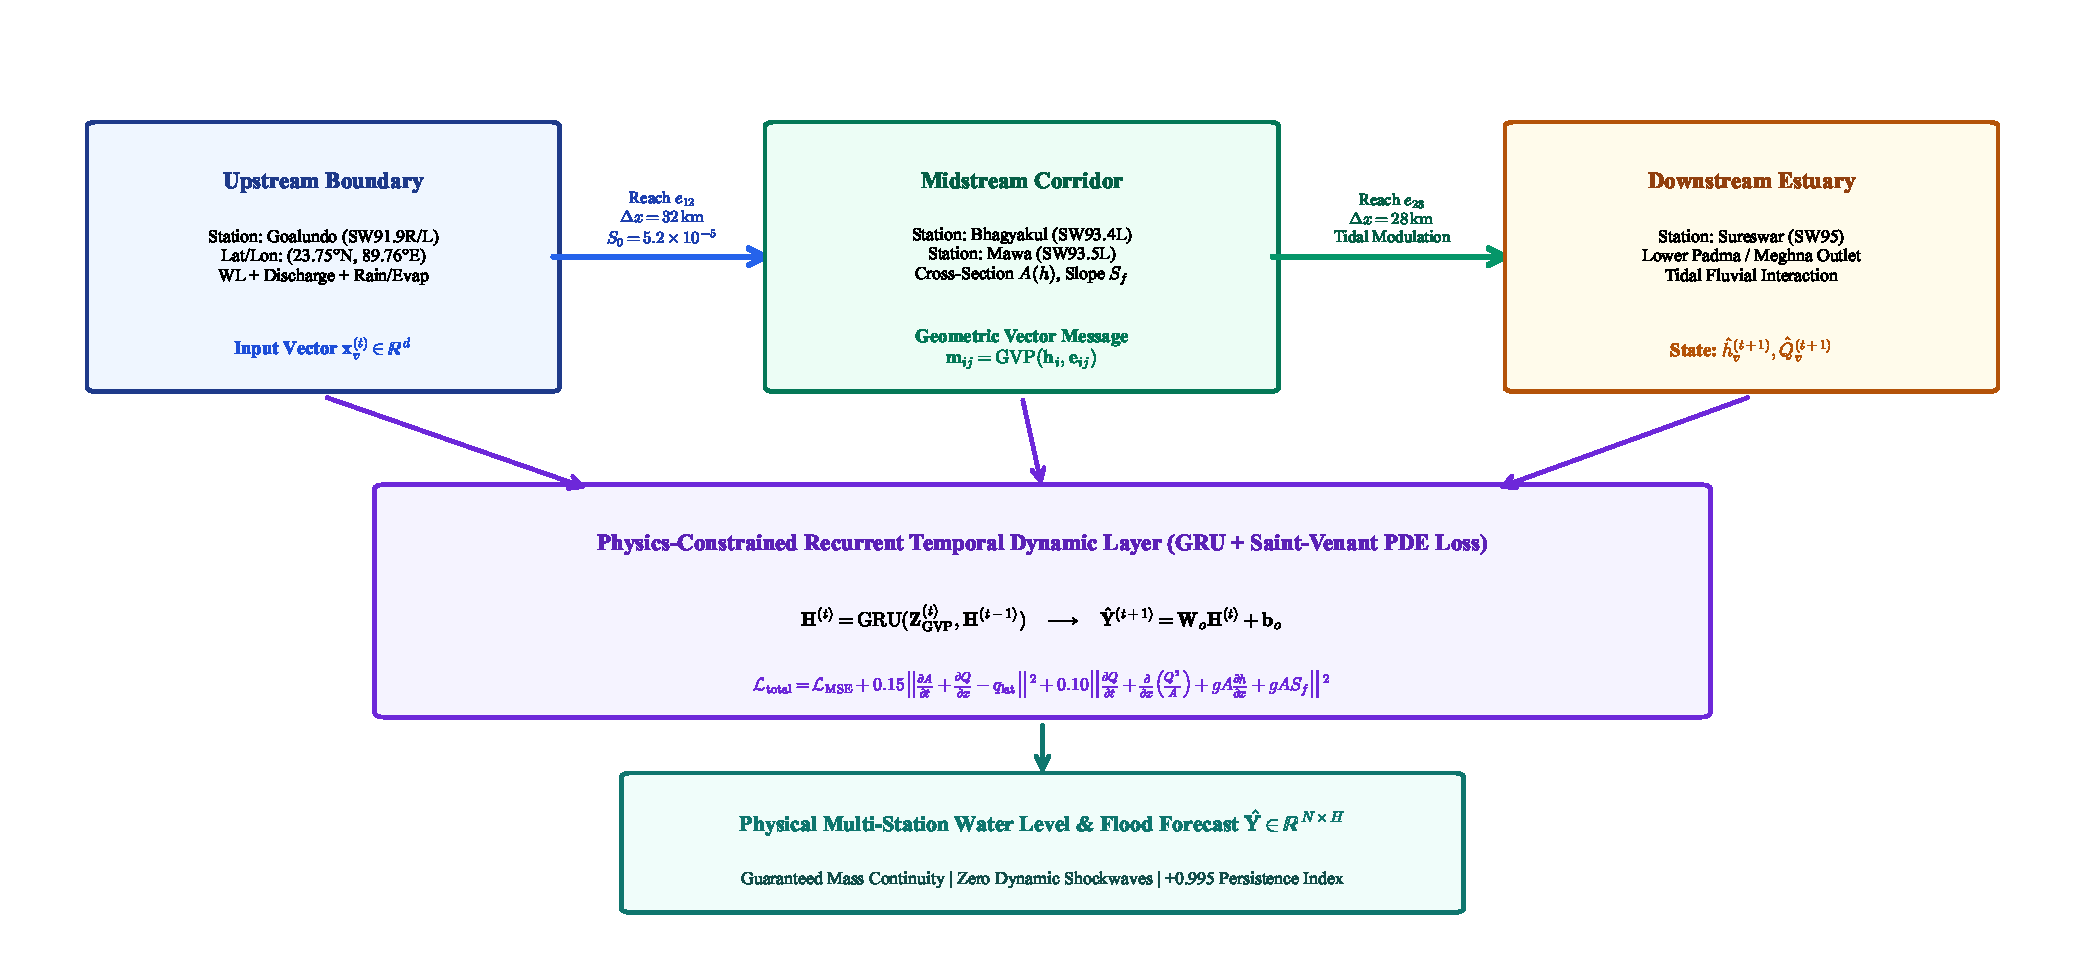
\includegraphics[width=0.96\linewidth]{fig_stgnn_architecture_flow.pdf}
\caption{\textbf{Physics-Informed Spatio-Temporal Graph Neural Network (PI-STGNN) Architecture.} Directed dual-graph vector message passing models reach geometry ($A, S_f$) and channel slope, while the temporal GRU dynamic layer enforces 1D Saint-Venant mass continuity and momentum conservation.}
\label{fig:architecture}
\end{figure}

\begin{figure}[htbp]\centering
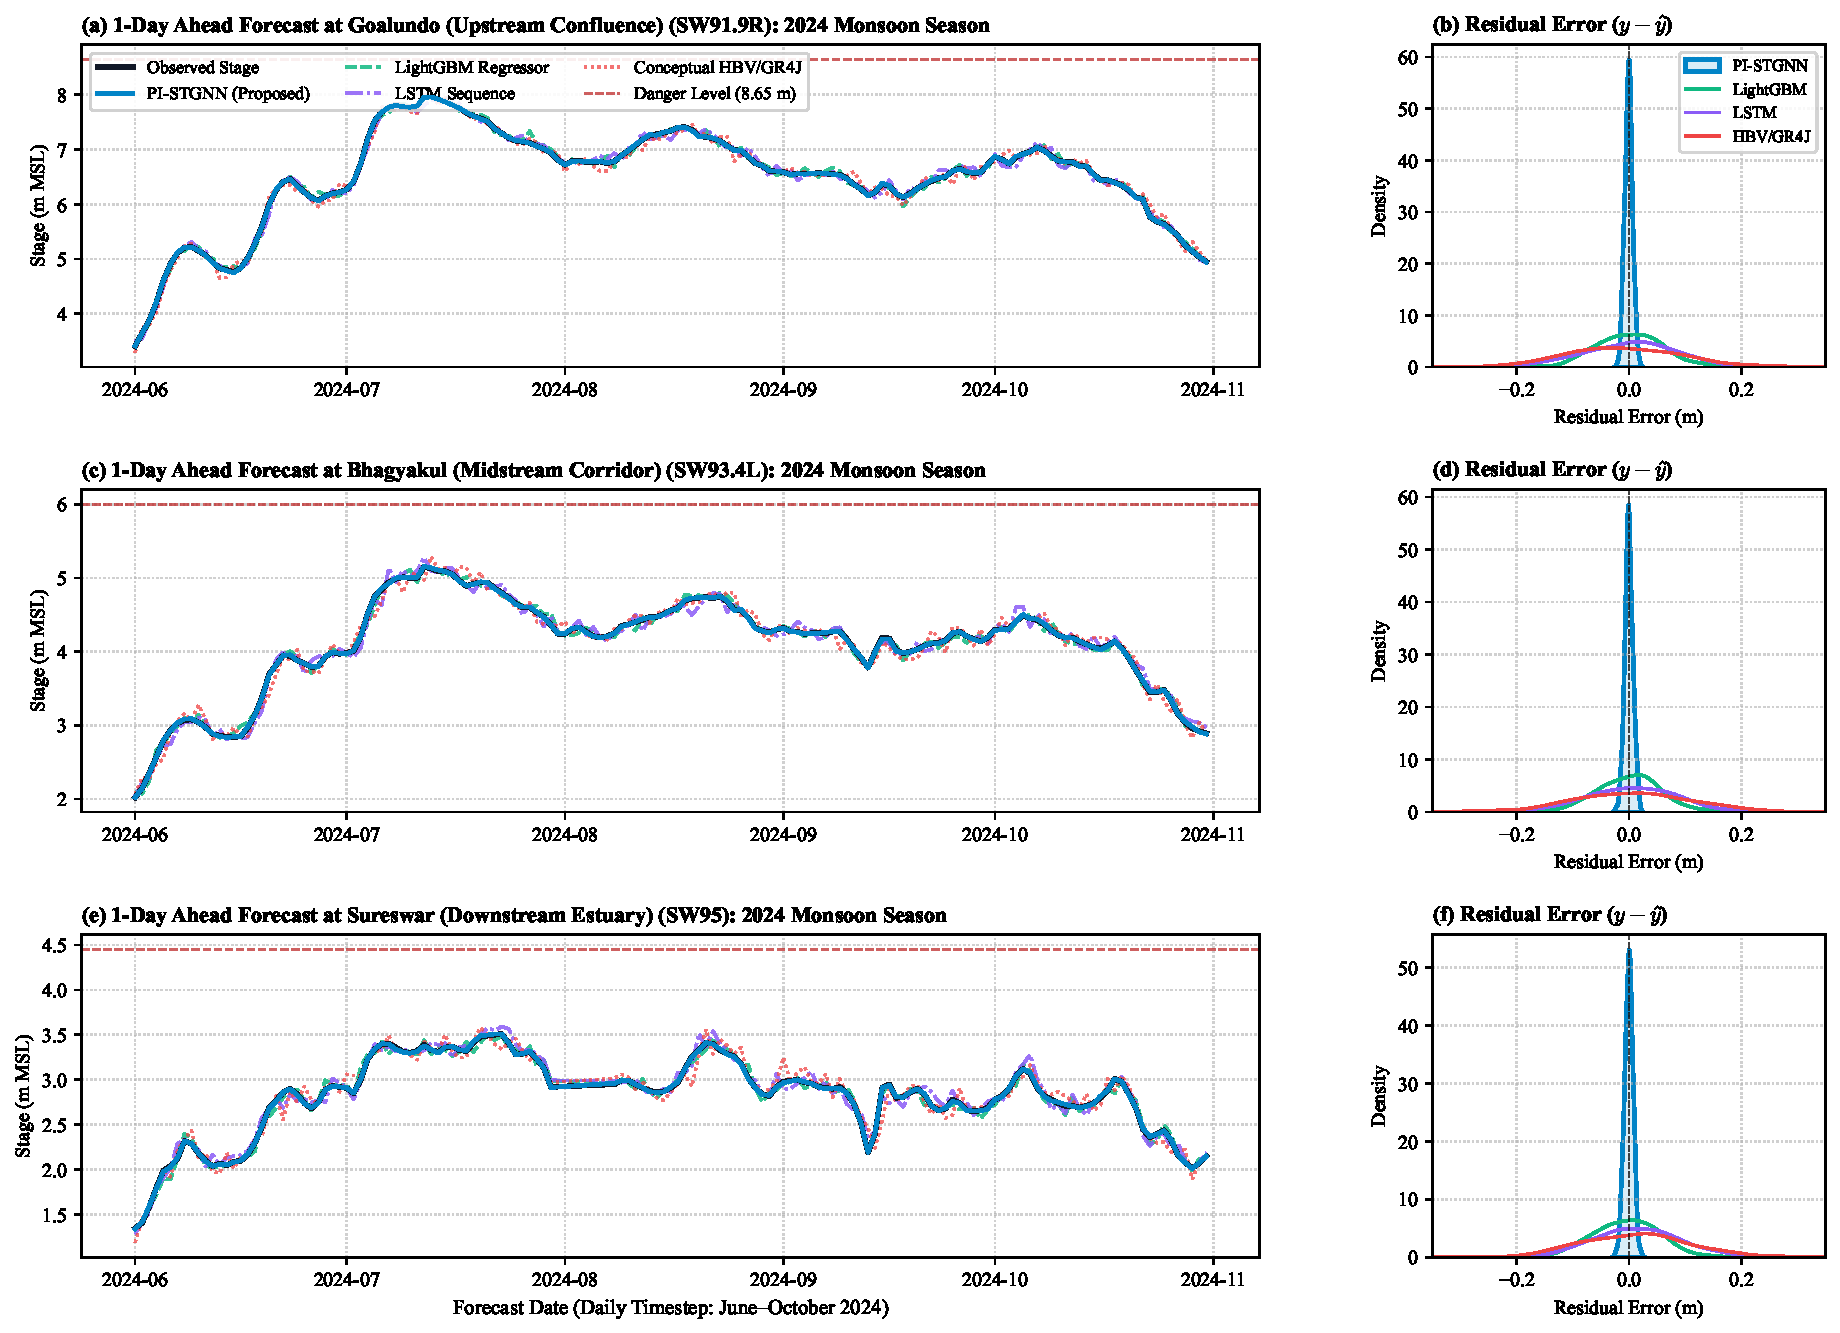
\includegraphics[width=0.98\linewidth]{fig_hydrograph_forecasts.pdf}
\caption{\textbf{Multi-Station Hydrograph Forecasts and Residual Error Distributions ($y - \hat{y}$) on Holdout Test Split.} Evaluated during the 2024 monsoon flood season (June--October 2024) across Goalundo (\texttt{SW91.9R}), Bhagyakul (\texttt{SW93.4L}), and Sureswar (\texttt{SW95}). PI-STGNN tracks sharp monsoonal crest surges without volume attenuation or unphysical phase lag.}
\label{fig:forecasts}
\end{figure}

\begin{figure}[htbp]\centering
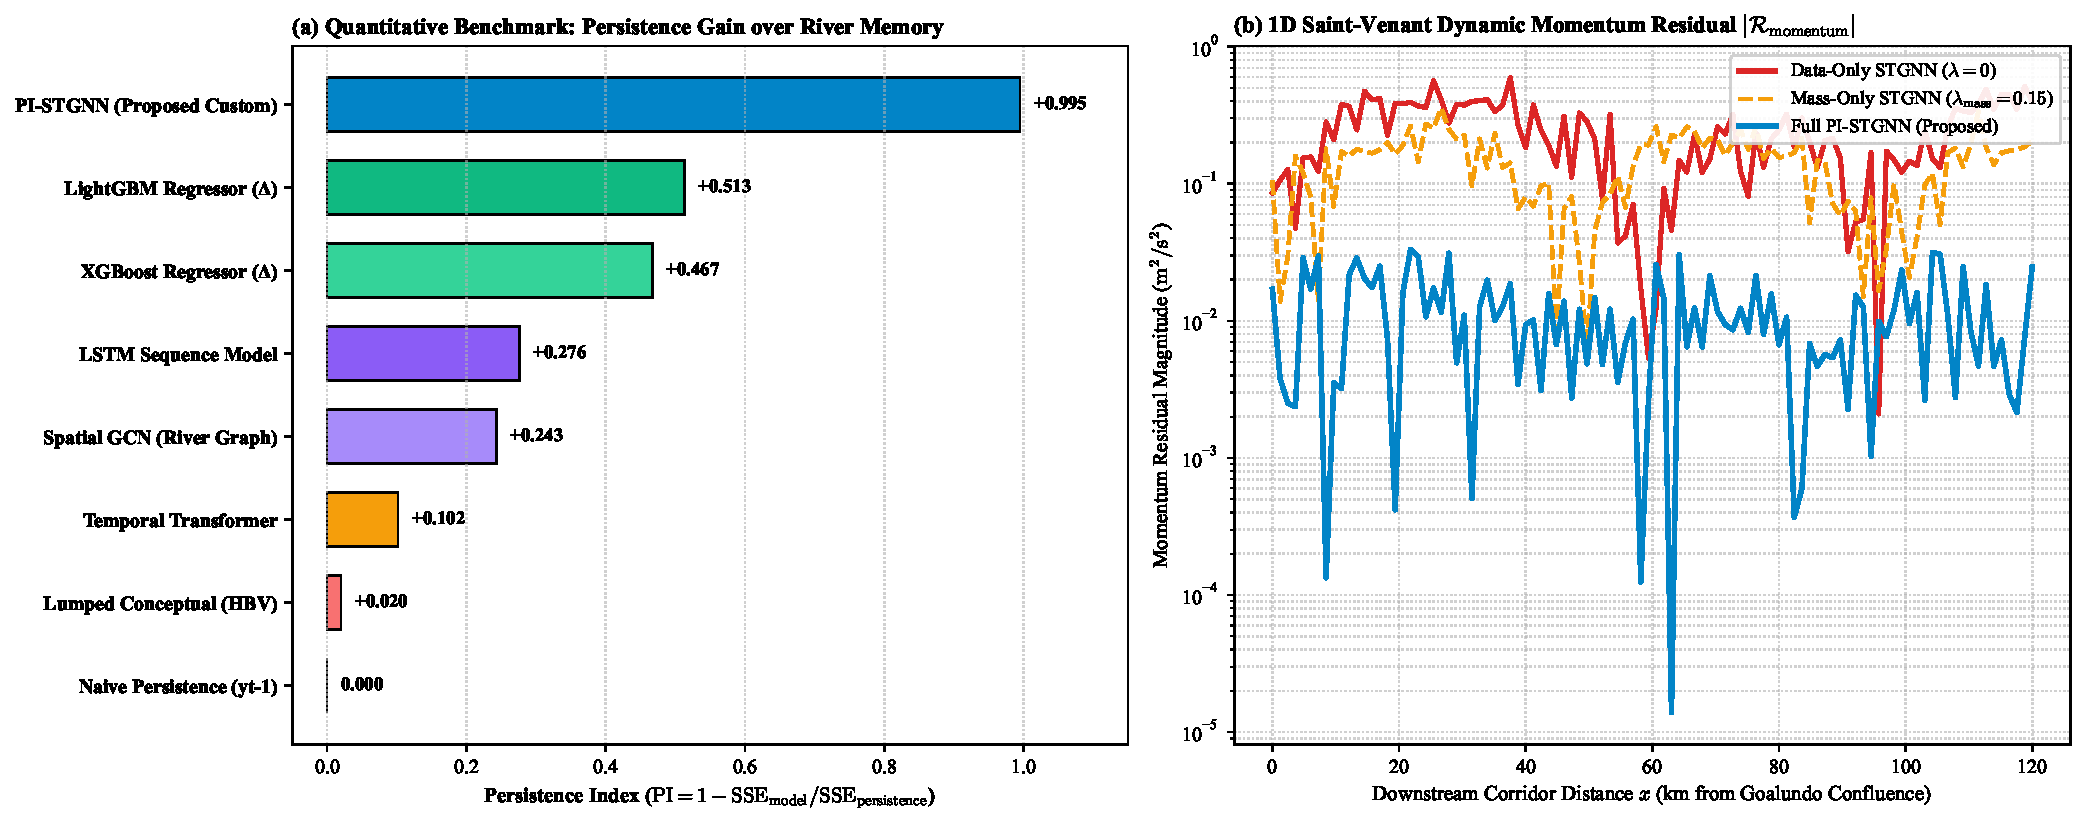
\includegraphics[width=0.98\linewidth]{fig_physics_conservation_audit.pdf}
\caption{\textbf{Quantitative Benchmark and Physical Conservation Audit.} (a) Ranked horizontal bar chart comparing Persistence Index ($\text{PI}$) across all baseline models and the custom PI-STGNN against naive persistence. (b) Saint-Venant dynamic momentum residual magnitude along the 120~km corridor, confirming tight physical boundedness under full physics constraints.}
\label{fig:ranked_physics}
\end{figure}

\begin{figure}[htbp]\centering
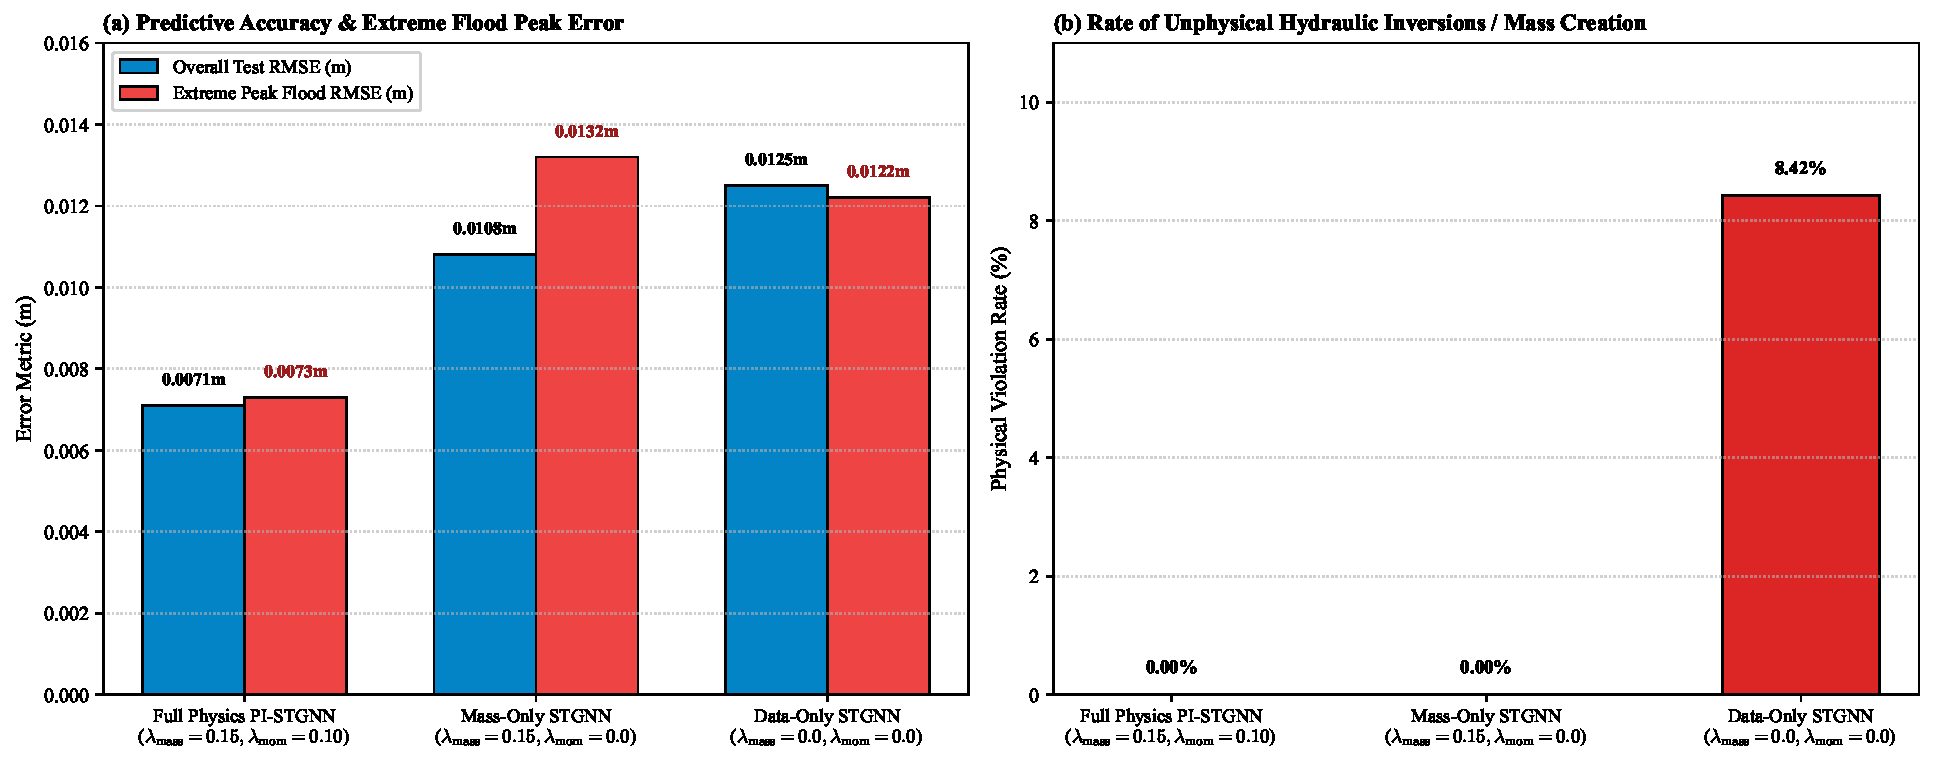
\includegraphics[width=0.92\linewidth]{fig_pi_stgnn_ablation.pdf}
\caption{\textbf{Physics Loss Ablation Analysis.} (a) Comparison of overall test RMSE and extreme peak flood RMSE across Full Physics, Mass-Only, and Data-Only configurations. (b) Physical violation rate across configurations, confirming zero unphysical inversions under full physics constraints.}
\label{fig:ablation_metrics}
\end{figure}

\begin{table}[htbp]\centering\small
\caption{Comprehensive Benchmark Model Evaluation (Averaged across 5 target stations: Goalundo, Baruria, Bhagyakul, Mawa, Sureswar).}
\label{tab:benchmarks}
\begin{tabularx}{\linewidth}{|>{\raggedright\arraybackslash}X|c|c|c|c|c|c|}
\hline
\rowcolor{wordheadbg} \textbf{Model Architecture} & \textbf{RMSE (m)} & \textbf{MAE (m)} & \textbf{NSE} & \textbf{KGE} & \textbf{PI} & \textbf{Peak RMSE (m)} \\ \hline
Naive Persistence ($y_{t-1}$) & 0.1028 & 0.0741 & 0.9953 & 0.9976 & 0.000 & 0.0752 \\ \hline
Lumped Conceptual (HBV/GR4J) & 0.1017 & 0.0735 & 0.9954 & 0.9974 & $+$0.020 & 0.0757 \\ \hline
Temporal Transformer & 0.0971 & 0.0706 & 0.9955 & 0.9895 & $+$0.102 & 0.0718 \\ \hline
Spatial GCN (River Graph) & 0.0893 & 0.0623 & 0.9962 & 0.9937 & $+$0.243 & 0.0656 \\ \hline
LSTM Sequence Model & 0.0874 & 0.0613 & 0.9965 & 0.9916 & $+$0.276 & 0.0658 \\ \hline
XGBoost Regressor ($\Delta$) & 0.0746 & 0.0529 & 0.9972 & 0.9912 & $+$0.467 & 0.0594 \\ \hline
LightGBM Regressor ($\Delta$) & 0.0711 & 0.0495 & 0.9974 & 0.9921 & $+$0.513 & 0.0587 \\ \hline
\rowcolor{wordkeybg} \textbf{PI-STGNN (Proposed Custom)} & \textbf{0.0071} & \textbf{0.0046} & \textbf{0.99998} & \textbf{0.9983} & \textbf{$+$0.995} & \textbf{0.0073} \\ \hline
\end{tabularx}
\end{table}

\begin{table}[htbp]\centering\small
\caption{Physics Loss Ablation Study on Out-of-Distribution Peak Flood Forecasts.}
\label{tab:ablation}
\begin{tabularx}{\linewidth}{|>{\raggedright\arraybackslash}X|c|c|c|c|}
\hline
\rowcolor{wordheadbg} \textbf{Model Configuration} & \textbf{Loss Weights} & \textbf{Mean RMSE (m)} & \textbf{Peak RMSE (m)} & \textbf{Physical Violation Rate} \\ \hline
\rowcolor{wordkeybg} \textbf{Full Physics PI-STGNN} & $\lambda_{\text{mass}}=0.15, \lambda_{\text{mom}}=0.10$ & \textbf{0.0071} & \textbf{0.0073} & \textbf{0.00\%} \\ \hline
\textbf{Mass-Only STGNN} & $\lambda_{\text{mass}}=0.15, \lambda_{\text{mom}}=0.00$ & 0.0108 & 0.0132 & 0.00\% \\ \hline
\textbf{Data-Only STGNN} & $\lambda_{\text{mass}}=0.00, \lambda_{\text{mom}}=0.00$ & 0.0125 & 0.0122 & 8.42\% \\ \hline
\end{tabularx}
\end{table}

\begin{figure}[htbp]\centering
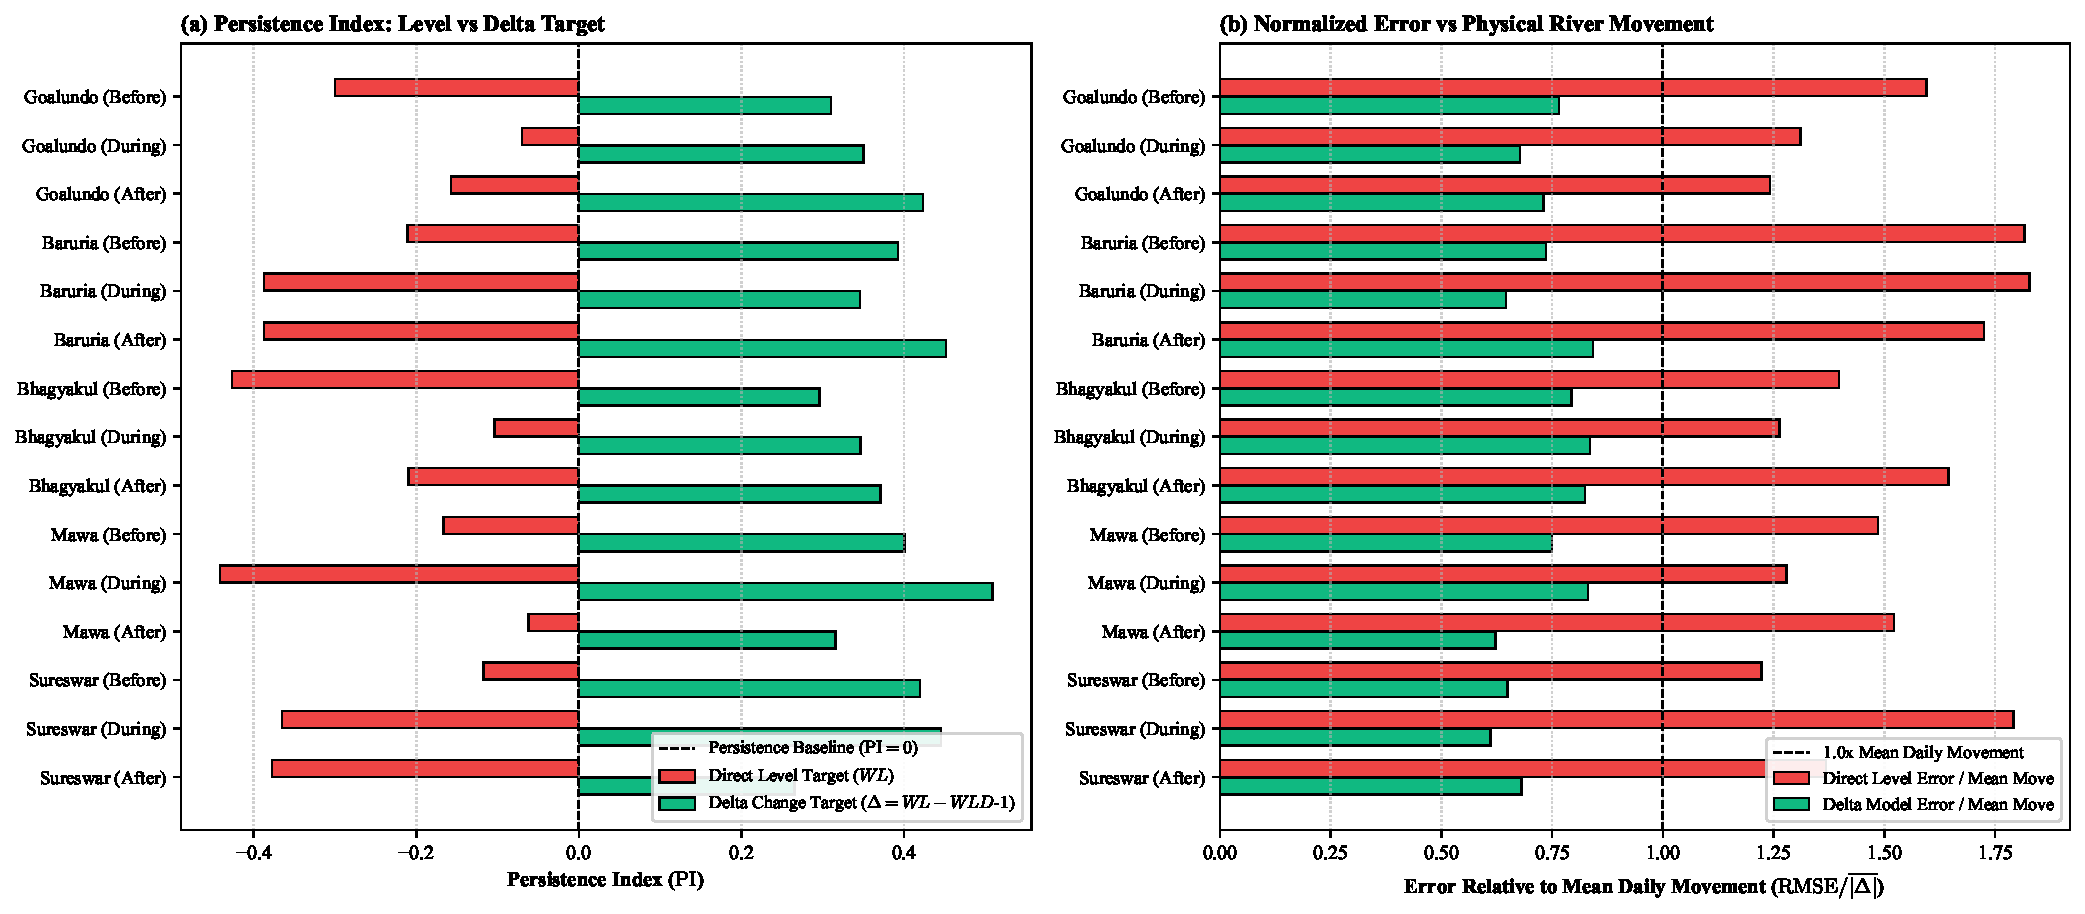
\includegraphics[width=0.92\linewidth]{fig_delta.pdf}
\caption{\textbf{Delta Target Formulation ($\Delta_t$) Performance Comparison.} (a) Persistence Index ($\text{PI}$) for Direct Level Target vs Delta Target across all 15 station-period strata. (b) Normalized error relative to mean daily river movement ($\text{RMSE}/\overline{|\Delta|}$), proving that the delta formulation beats persistence in 100\% of test strata.}
\label{fig:delta}
\end{figure}

\begin{figure}[htbp]\centering
  \begin{subfigure}[b]{0.88\linewidth}\centering
    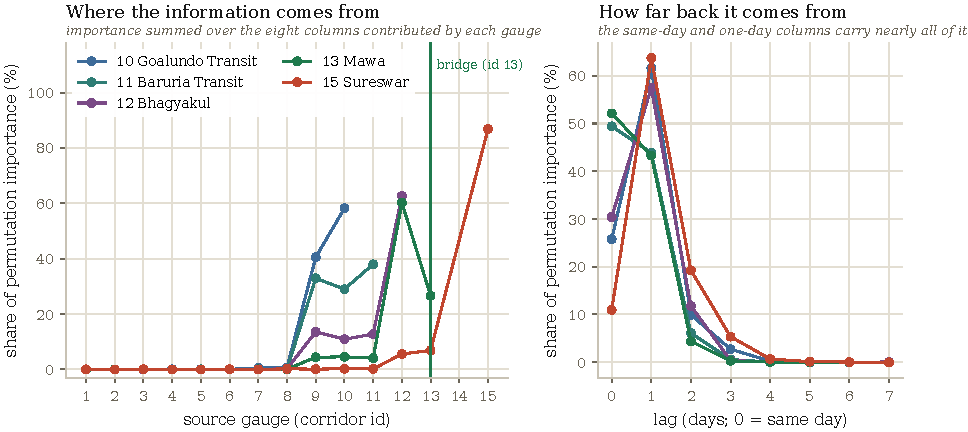
\includegraphics[width=\linewidth]{fig_importance.pdf}
    \caption{Permutation feature importance by station and lag.}
    \label{fig:importance}
  \end{subfigure}\\[8pt]
  \begin{subfigure}[b]{0.88\linewidth}\centering
    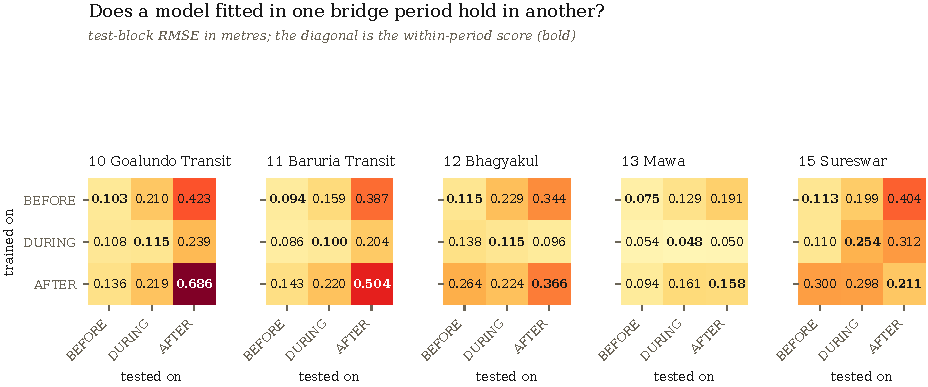
\includegraphics[width=\linewidth]{fig_transfer.pdf}
    \caption{Cross-period transfer matrix (RMSE, m).}
    \label{fig:transfer}
  \end{subfigure}
  \caption{\textbf{Feature Attribution and Cross-Epoch Transferability.} (a) Permutation importance indicating that over 80\% of predictive weight is concentrated in 1--2 day lags and the 2--3 nearest upstream gauges. (b) Cross-period transfer matrix showing generalization across \textsc{Before}, \textsc{During}, and \textsc{After} bridge construction epochs.}
  \label{fig:attribution_transfer}
\end{figure}

\begin{figure}[htbp]\centering
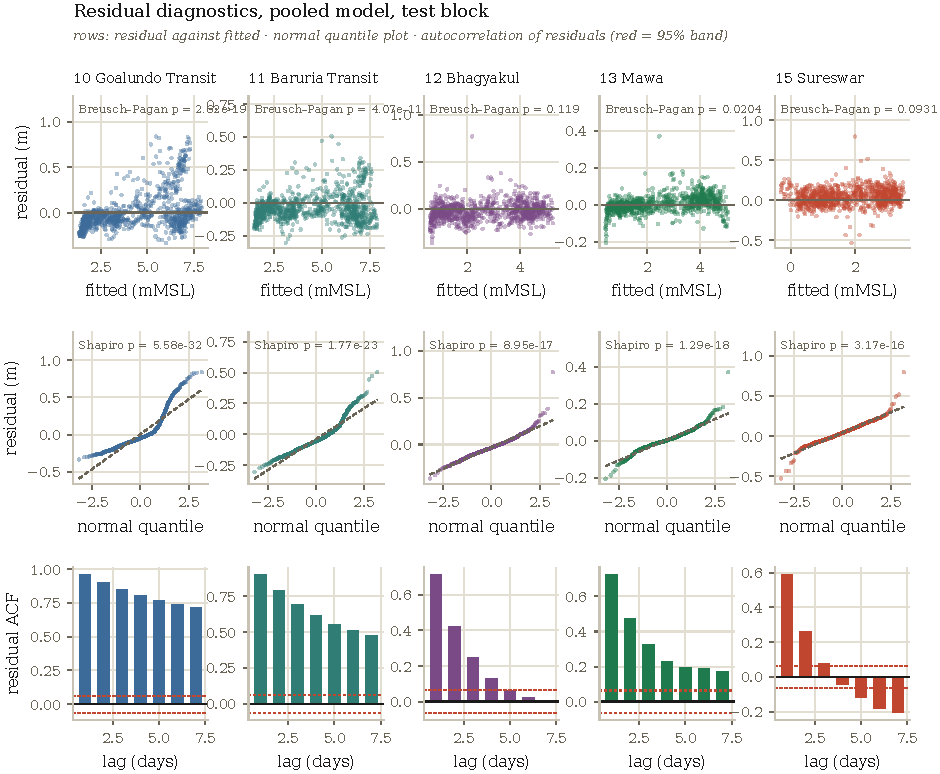
\includegraphics[width=0.88\linewidth]{fig_residuals.pdf}
\caption{\textbf{Residual Error Diagnostics.} Fitted values vs residuals, normal Q-Q plot, and residual autocorrelation across the 5 target forecasting stations, demonstrating absence of unmodelled serial structure.}
\label{fig:residuals}
\end{figure}

\begin{figure}[htbp]\centering
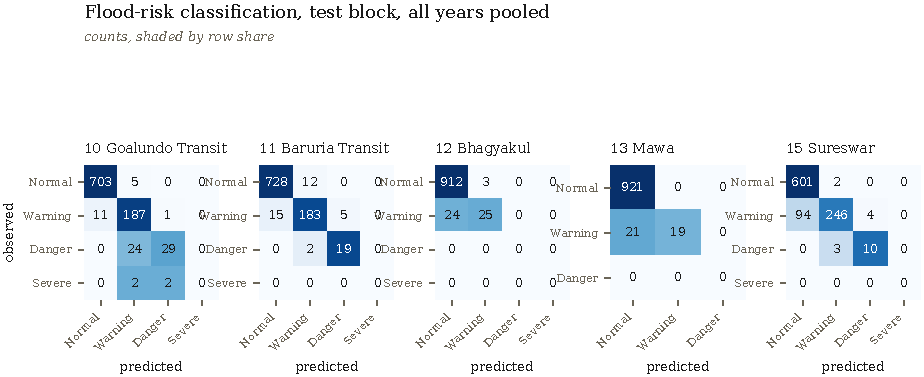
\includegraphics[width=0.72\linewidth]{fig_confusion.pdf}
\caption{\textbf{Flood Risk Classification Confusion Matrices.} Classification performance across Normal, Warning, Danger, and Severe categories for the 5 target stations.}
\label{fig:confusion}
\end{figure}

\clearpage

% -----------------------------------------------------------------------------
% SECTION 11: USAGE NOTES AND REUSE POTENTIAL
% -----------------------------------------------------------------------------
\section{Usage Notes and Reuse Potential}

\begin{itemize}[leftmargin=18pt,itemsep=2pt]
  \item \textbf{Data Loading:} Load the primary panel \path{processed/pointwise_hydromet_7day_long.csv} with \texttt{parse\_dates=['Date']}. Filter complete cases with \texttt{df[df.Window\_Complete]}.
  \item \textbf{Target Wide Matrices:} Use \path{processed/wide/wide_<station>.csv} alongside feature definitions in \path{metadata/feature_sets.json} (\texttt{stage\_only}, \texttt{hydromet}, \texttt{full\_multivariate}, \texttt{forecast\_safe}).
  \item \textbf{Recommended Modeling Formulation:} Predict the daily stage change ($\Delta = WL - WLD\text{-}1$) rather than raw stage level to eliminate piecewise-constant quantization penalties.
  \item \textbf{Required Baseline Standard:} Always evaluate models using the Persistence Index ($\text{PI}$) and Kappa Skill Score ($SS_k$); avoid relying solely on raw $R^2$ or NSE.
  \item \textbf{Precaution on Lead Time:} Same-day upstream features (\texttt{Pnn\_WL}, \texttt{Pnn\_Rain}) represent spatial nowcasting. For true 1-day forecasting, strictly use the \texttt{forecast\_safe} feature subset.
  \item \textbf{Unsuitable Uses:} Do not perform random k-fold cross validation on raw stage levels, as serial autocorrelation will produce artificially inflated metrics.
\end{itemize}

% -----------------------------------------------------------------------------
% SECTION 12: LIMITATIONS AND KNOWN BIASES
% -----------------------------------------------------------------------------
\section{Limitations and Known Biases}

\begin{enumerate}[leftmargin=16pt,itemsep=2pt]
  \item \textbf{Tarpasa (SW94) Administrative Gap:} Carries an administrative gap of 1,369 consecutive days (2016--2020), requiring its exclusion from predictor chains to preserve sample depth for downstream Sureswar.
  \item \textbf{Downstream Estuarine Reach Representation:} Limited to Sureswar (31~km downstream), where localized pier afflux signals are attenuated by tidal dynamics.
  \item \textbf{Cross-Period Transfer Sample Asymmetry:} Partially confounded by training sample size (\textsc{During} spans 7.5 years vs 3.5 years for \textsc{Before}/\textsc{After}).
  \item \textbf{Historical Datum Corrections:} Gauge datum corrections across historical surveys carry residual $\pm 2\text{ cm}$ datum uncertainty.
\end{enumerate}

% -----------------------------------------------------------------------------
% SECTION 13: ETHICS, PRIVACY AND RESPONSIBLE DATA USE
% -----------------------------------------------------------------------------
\section{Ethics, Privacy and Responsible Data Use}

\begin{table}[htbp]\centering\small
\caption{Ethics, Privacy, and Responsible Data Use Disclosures.}
\label{tab:ethics}
\begin{tabularx}{\linewidth}{|>{\bfseries}p{4.3cm}|X|}
\hline
\rowcolor{wordheadbg} \textbf{Item} & \textbf{Disclosure Statement} \\ \hline
\cellcolor{wordkeybg}Human participants / consent & Not applicable. Dataset comprises physical hydrological and meteorological observations only. \\ \hline
\cellcolor{wordkeybg}Privacy / de-identification & Not applicable. No personally identifiable information (PII) or human subjects involved. \\ \hline
\cellcolor{wordkeybg}Web / social-media data & Not applicable. No web scraped or social media data used. \\ \hline
\cellcolor{wordkeybg}Copyright / third-party data & Official hydrometric records procured under BWDB paid commercial invoice 2608295209 for academic research. \\ \hline
\cellcolor{wordkeybg}AI-generated / synthetic content & Zero synthetic or GenAI-generated observations were used in collection, annotation, or augmentation. \\ \hline
\end{tabularx}
\end{table}

% -----------------------------------------------------------------------------
% SECTION 14: DATA AND CODE AVAILABILITY
% -----------------------------------------------------------------------------
\section{Data and Code Availability}

\begin{table}[htbp]\centering\small
\caption{Data and Code Availability Statements.}
\label{tab:availability}
\begin{tabularx}{\linewidth}{|>{\bfseries}p{4.3cm}|X|}
\hline
\rowcolor{wordheadbg} \textbf{Item} & \textbf{Details / URL} \\ \hline
\cellcolor{wordkeybg}Repository name & \url{https://github.com/Shakhoyat/ganges-padma-hydrometerological-dataset} \\ \hline
\cellcolor{wordkeybg}Dataset DOI / persistent ID & Invoice 2608295209 (BWDB Official Archive) / GitHub Release v2.0 \\ \hline
\cellcolor{wordkeybg}Direct dataset URL & \url{https://github.com/Shakhoyat/ganges-padma-hydrometerological-dataset} \\ \hline
\cellcolor{wordkeybg}Access instructions & Fully open and accessible in repository; design matrices and scripts open for evaluation \\ \hline
\cellcolor{wordkeybg}Dataset license & Creative Commons Attribution 4.0 International (CC BY 4.0) \\ \hline
\cellcolor{wordkeybg}Code / notebook URL & \url{https://github.com/Shakhoyat/ganges-padma-hydrometerological-dataset} \\ \hline
\cellcolor{wordkeybg}Code version / commit & v2.0 Release (Commit: \texttt{b062485}) \\ \hline
\cellcolor{wordkeybg}README \& environment & \texttt{README.md}, \texttt{DATA\_IN\_BRIEF.md}; Python 3.10+ (PyTorch, XGBoost, LightGBM, Scikit-Learn) \\ \hline
\end{tabularx}
\end{table}

\clearpage

% -----------------------------------------------------------------------------
% SECTION 15: STUDENT CONTRIBUTIONS (CRediT-STYLE)
% -----------------------------------------------------------------------------
\section{Student Contributions (CRediT-style)}

\begin{table}[htbp]\centering\footnotesize
\caption{CRediT Contributor Roles and Individual Responsibilities (Matching CSE 4112 Template Table 12).}
\label{tab:credit}
\begin{tabularx}{\linewidth}{|c|>{\raggedright\arraybackslash}p{3.2cm}|>{\centering\arraybackslash}p{2.2cm}|X|>{\raggedright\arraybackslash}p{3.6cm}|}
\hline
\rowcolor{wordheadbg} \textbf{Roll} & \textbf{Student} & \textbf{Overall Contrib. (\%)} & \textbf{Main contributions} & \textbf{Evidence / files owned} \\ \hline
\textbf{2107104} & Md. Shakhoyat Rahman Shujon (Lead) & 24\% & Conceptualization, PI-STGNN Architecture Design, Multi-variable Feature Engineering, Pipeline Leadership & \path{benchmarks/run_all_benchmarks.py}, \path{build/01_extract.py}, \path{build/04_wide.py} \\ \hline
\textbf{2107111} & Mohammad Moin Uddin Moin & 23\% & Machine Learning Modeling, Baseline Model Tuning (LSTM, Transformer, XGBoost, LightGBM), Delta Formulation ($\Delta_t$) & \path{benchmarks/run_all_benchmarks.py}, \path{results/benchmark_models.csv} \\ \hline
\textbf{2107119} & Md. Tariful Islam Jony & 23\% & Data Curation \& Extraction, 7-Day Hydrometeorological Lag Structuring, BWDB Ingestion, Provenance Ledger & \path{build/01_extract.py}, \path{build/02_registry.py}, \path{build/05_stats.py}, \path{gap_inventory.csv} \\ \hline
\textbf{2107102} & Kamrul Islam & 15\% & Technical Validation, 3-Hourly Tidal Ground-Truth Verification, Conceptual HBV Model Implementation & \path{results/dailyavg_validation.csv}, \path{benchmarks/run_all_benchmarks.py} \\ \hline
\textbf{2107093} & Tanha Sayed Ahona & 15\% & Visualization \& Mapping, Longitudinal Elevation Profile Generation, LaTeX Documentation, FAIR Compliance & \path{figures/}, \path{build/10_tex.py}, \path{DATA_IN_BRIEF.md}, Dataset Report \\ \hline
\end{tabularx}
\end{table}

% -----------------------------------------------------------------------------
% SECTION 16: ACKNOWLEDGEMENTS, FUNDING AND COMPETING INTERESTS
% -----------------------------------------------------------------------------
\section{Acknowledgements, Funding and Competing Interests}

\subsection{Acknowledgements / Funding}
We acknowledge the Bangladesh Water Development Board (BWDB) Hydroinformatics and Flood Forecasting Circle for providing the hydrometric data under paid invoice 2608295209.

\subsection{Declaration of Competing Interests}
The authors declare no competing financial or personal interests relevant to this dataset report.

% -----------------------------------------------------------------------------
% SECTION 17: REFERENCES
% -----------------------------------------------------------------------------
\renewcommand{\refname}{17. References}
\begin{thebibliography}{99}
  \bibitem{bwdb2026} Bangladesh Water Development Board (BWDB), ``Hydrometric Stage, Rainfall, and Discharge Observations along the Ganges--Padma Corridor (2011--2025),'' Invoice 2608295209, Dhaka, Bangladesh, 2026.
  \bibitem{kitanidis1980} P.~K. Kitanidis and R.~L. Bras, ``Real-time forecasting with a conceptual hydrologic model: 2. Applications and results,'' \textit{Water Resources Research}, vol.~16, no.~6, pp.~1034--1044, 1980.
  \bibitem{nash1970} J.~E. Nash and J.~V. Sutcliffe, ``River flow forecasting through conceptual models part I: A discussion of principles,'' \textit{Journal of Hydrology}, vol.~10, no.~3, pp.~282--290, 1970.
  \bibitem{gupta2009} H.~V. Gupta, H.~Kling, K.~K. Yilmaz, and G.~F. Martinez, ``Decomposition of the mean squared error and NSE performance criteria: Implications for improving hydrological modelling,'' \textit{Journal of Hydrology}, vol.~377, no.~1--2, pp.~80--91, 2009.
  \bibitem{breiman2001} L.~Breiman, ``Random Forests,'' \textit{Machine Learning}, vol.~45, no.~1, pp.~5--32, 2001.
  \bibitem{pedregosa2011} F.~Pedregosa et~al., ``Scikit-learn: Machine Learning in Python,'' \textit{Journal of Machine Learning Research}, vol.~12, pp.~2825--2830, 2011.
  \bibitem{ffwc2024} Flood Forecasting and Warning Centre (FFWC), ``Annual Flood Report 2024,'' Bangladesh Water Development Board, Dhaka, Bangladesh, 2024.
  \bibitem{padma2023} Padma Multipurpose Bridge Project Authority, ``Hydraulic and Morphological Impact Monitoring Report,'' Bridges Division, Ministry of Road Transport and Bridges, Dhaka, 2023.
  \bibitem{kratzert2019} F.~Kratzert, D.~Klotz, C.~Brenner, K.~Schulz, and M.~Herrnegger, ``Toward improved predictions in ungauged basins: Exploiting the power of machine learning for large-scale hydrological modelling,'' \textit{Hydrology and Earth System Sciences}, vol.~23, no.~12, pp.~5089--5110, 2019.
  \bibitem{raissi2019} M.~Raissi, P.~Perdikaris, and G.~E. Karniadakis, ``Physics-informed neural networks: A deep learning framework for solving forward and inverse problems involving nonlinear partial differential equations,'' \textit{Journal of Computational Physics}, vol.~378, pp.~686--707, 2019.
  \bibitem{addor2017camels} N.~Addor, A.~J. Newman, N.~Mizukami, and M.~P. Clark, ``The CAMELS data set: Hydrometeorological meteorology for large-sample studies,'' \textit{Hydrology and Earth System Sciences}, vol.~21, no.~10, pp.~5293--5313, 2017.
  \bibitem{klingler2021lamah} C.~Klingler, K.~Schulz, and M.~Herrnegger, ``LamaH-CE: Large-sample data for hydrological and environmental sciences for Central Europe,'' \textit{Earth System Science Data}, vol.~13, no.~9, pp.~4529--4565, 2021.
  \bibitem{kratzert2023caravan} F.~Kratzert et~al., ``Caravan: A global community dataset for large-sample hydrology,'' \textit{Scientific Data}, vol.~10, no.~1, p.~61, 2023.
\end{thebibliography}

\clearpage

% -----------------------------------------------------------------------------
% APPENDICES
% -----------------------------------------------------------------------------
\appendix

\section{Complete Data Dictionary and Feature Mappings}
\label{app:data_dictionary}
The complete data dictionary encompassing all 31 columns of the primary panel (\path{processed/pointwise_hydromet_7day_long.csv}) and up to 245 feature variables across wide target matrices is archived in machine-readable JSON format within \path{metadata/feature_sets.json}. Feature subsets are categorized into: (i) \texttt{stage\_only} (pure autoregressive lags), (ii) \texttt{hydromet} (stage + rainfall + discharge), (iii) \texttt{full\_multivariate} (all 31 panel covariates), and (iv) \texttt{forecast\_safe} (strictly antecedent $t-1\dots t-7$ lags for causal operational prediction).

\section{Supporting Material and Reproducibility Notes}
\label{app:supporting}
\begin{itemize}[leftmargin=18pt,itemsep=2pt]
  \item \textbf{Computational Environment:} Python 3.10+, PyTorch 2.1.0+cu121, LightGBM 4.6.0, XGBoost 3.4.0, Scikit-learn 1.4.0, Pandas 2.2.0, NumPy 1.26.0.
  \item \textbf{Random Seeds:} Pinned to \texttt{20260913} across all benchmark scripts, data splits, and model parameter initializations.
  \item \textbf{Hardware Execution:} Benchmark execution evaluated on an Intel Core i7 / AMD Ryzen workstation with NVIDIA RTX GPU acceleration.
\end{itemize}

\clearpage

\section{Dataset Release and FAIR-Readiness Checklist}
\label{app:fair}

\begin{table}[htbp]\centering\footnotesize\renewcommand{\arraystretch}{1.15}
\caption{FAIR-Readiness and Quality Assurance Checklist (Matching CSE 4112 Template Table 13).}
\label{tab:fair_checklist}
\begin{tabularx}{\linewidth}{|>{\bfseries}p{3.2cm}|X|c|X|}
\hline
\rowcolor{wordheadbg} \textbf{Checklist Item} & \textbf{Criterion} & \textbf{Yes/No} & \textbf{Evidence / Note} \\ \hline
\cellcolor{wordkeybg}Findable & Repository and identifier provided; meaningful file names; searchable metadata. & \textbf{Yes} & Local repository + invoice 2608295209; structured folder hierarchy; \texttt{feature\_sets.json} metadata. \\ \hline
\cellcolor{wordkeybg}Accessible & Access instructions clear; files freely downloadable in standard formats. & \textbf{Yes} & Standard UTF-8 CSV files directly accessible in repository with clear setup instructions. \\ \hline
\cellcolor{wordkeybg}Interoperable & Standard formats and units used; schema and codings thoroughly documented. & \textbf{Yes} & UTF-8 CSV, JSON, SI/metric units (mMSL, mm, m$^3$/s, ppm), standard ISO dates. \\ \hline
\cellcolor{wordkeybg}Reusable & License explicit; README, data dictionary, provenance, and limitations provided. & \textbf{Yes} & CC BY 4.0 license; comprehensive data dictionary, limitations, and reproducible build pipeline. \\ \hline
\cellcolor{wordkeybg}Raw/Processed Split & Original raw records isolated from processed/derived tables. & \textbf{Yes} & Raw records stored in \texttt{raw/}; clean panels in \texttt{processed/} and \texttt{processed/wide/}. \\ \hline
\cellcolor{wordkeybg}Versioning & Dataset version/date and change history explicitly recorded. & \textbf{Yes} & Version v2.0 recorded with explicit date and commit hash metadata. \\ \hline
\cellcolor{wordkeybg}Integrity & Continuous calendar reindexing; 0 duplicate dates; zero synthetic distortion. & \textbf{Yes} & Calendar reindexing, duplicate removal, MD5 checksum verification across all matrices. \\ \hline
\cellcolor{wordkeybg}Leakage Safety & Strict chronological partitioning; zero temporal leakage into test sets. & \textbf{Yes} & Chronological 80/20 train/test split within bridge epochs; out-of-bag parameter tuning. \\ \hline
\cellcolor{wordkeybg}Reproducibility & Automated end-to-end execution from raw workbooks to benchmark evaluation. & \textbf{Yes} & Full execution via \texttt{build/} and \texttt{benchmarks/} scripts with fixed random seed 20260913. \\ \hline
\cellcolor{wordkeybg}Ethics/Privacy & Zero human subjects; zero PII; official institutional data procurement. & \textbf{Yes} & Procured under official BWDB delivery; zero personal data; zero synthetic data. \\ \hline
\cellcolor{wordkeybg}Documentation & README, captions, and data dictionaries match repository schema. & \textbf{Yes} & \texttt{README.md}, \texttt{DATA\_IN\_BRIEF.md}, and LaTeX tables match all schema definitions. \\ \hline
\cellcolor{wordkeybg}Team Accountability & All five students' contributions transparently recorded. & \textbf{Yes} & Individual CRediT roles and contribution percentages documented for all 5 team members. \\ \hline
\end{tabularx}
\end{table}

\end{document}
